\input{../../common/slide-common-header.tex}

\newcommand{\orgNum}{0}
\newcommand{\orgTopic}{org meeting}
\newcommand{\orgKey}{syllabus, contacts}

\newcommand{\introNum}{1}
\newcommand{\introTopic}{introduction to multithreading}
\newcommand{\introKey}{concurrency, parallelism, agents, threads, scheduler, Amdahl's law, race condition, deadlock, wait-for graph}

\newcommand{\basicNum}{2}
\newcommand{\basicTopic}{basic concepts}
\newcommand{\basicKey}{mutex, acquisition order, reentrancy, fairness, data locking, code locking, signalling, condition variable, lost signal, spurious wakeup}

\newcommand{\syncPrimitivesNum}{3}
\newcommand{\syncPrimitivesTopic}{advanced synchronization primitives}
\newcommand{\syncPrimitivesKey}{monitor, latch, barrier, thundering herd, semaphore, read-write lock, thread pool, executor, producer-consumer, fork-join, load balancing}

\newcommand{\patternsNum}{4}
\newcommand{\patternsTopic}{advanced synchronization concepts}
\newcommand{\patternsKey}{interruption, cancellation, partitioning, privatization, replication, thread-local, ownership}

\newcommand{\extraBasicsNum}{5}
\newcommand{\extraBasicsTopic}{additional topics of practical concurrency}
\newcommand{\extraBasicsKey}{documenting protocols and classes, checking concurrent invariants, stress testing, execution trace analysis, estimating required testing effort, static and dynamic checks, scheduling randomization, model checking}

\newcommand{\foundationsNum}{6}
\newcommand{\foundationsTopic}{theoretical foundations of concurrency}
\newcommand{\foundationsKey}{timeline, events, precedence, 2-thread mutual exclusion, deadlock freedom, starvation freedom, N-thread mutual exclusion, sequential objects and specifications, concurrent objects, linearizability}

\newcommand{\foundationsPlusNum}{7}
\newcommand{\foundationsPlusTopic}{progress guarantees, concurrent operations hierarchy, consensus number}
\newcommand{\foundationsPlusKey}{obstruction-free, lock-free, wait-free, safe register, regular register, atomic register, register snapshot, consensus number}

\newcommand{\atomicsNum}{8}
\newcommand{\atomicsTopic}{introduction to atomics}
\newcommand{\atomicsKey}{read-modify-write, get-and-add, compare-and-swap, spin lock, lock-free stack, ABA problem}

% TODO: taxonomy of queues, 

\newcommand{\cacheCoherencyNum}{9}
\newcommand{\cacheCoherencyTopic}{cache coherency}
\newcommand{\cacheCoherencyKey}{cache memory hierarchy, cache coherency protocol, store-buffer, load-buffer, invalidate-queue, memory barrier, hardware memory model, weak memory model, litmus tests}

\newcommand{\langMMNum}{10}
\newcommand{\langMMTopic}{language memory model}
\newcommand{\langMMKey}{compiler optimizations, compiler barriers, language memory model, strict consistency, threads cannot be implemented as a library, visibility, volatile}

\newcommand{\advancedConcurrencyNum}{11}
\newcommand{\advancedConcurrencyTopic}{advanced locking}
\newcommand{\advancedConcurrencyKey}{Anderson Queue Lock, CLH, MCS, check-then-act, spin-then-park}

% TODO: work distribution, work stealing, taxonomy of parallel problems, single LIFO cell optimization, RAT

\newcommand{\userSpaceThreadingNum}{12}
\newcommand{\userSpaceThreadingTopic}{user-space threading}
\newcommand{\userSpaceThreadingKey}{berkley socket, blocking and non-blocking IO, callback-hell, async-await, continuation-passing-style, fibers/coroutines/green threads, stackful vs stackless}


\newcommand{\designNum}{13}
\newcommand{\designTopic}{designing concurrent systems}
\newcommand{\designKey}{park/unpark, synchronizer, futex/wait-on-address, plan9 approach, race-finders, ForkJoinPool/CoroutineCarriers/UIthread, observability, structured concurrency}

\newcommand{\frameworksAndDistributedNum}{14}
\newcommand{\frameworksAndDistributedTopic}{multi-agent systems}
\newcommand{\frameworksAndDistributedKey}{auto-parallelization languages and frameworks, semi-automatic synchronization, distributed systems, consensus protocols}



\title[]{Lecture \advancedConcurrencyNum: \advancedConcurrencyTopic}
\subtitle[]{\advancedConcurrencyKey}
\author[]{Alexander Filatov\\ filatovaur@gmail.com}

\date{}

\begin{document}

\begin{frame}
  \titlepage
  \url{https://github.com/Svazars/parallel-programming/blob/main/slides/pdf/l11.pdf}
\end{frame}


\begin{frame}{In previous episodes}

Hardware optimizations
\begin{itemize}
 \item Store buffering, Load buffering, Invalidate Queues, Interconnect topology
\end{itemize}

Compiler optimizations
\begin{itemize}
 \item reorder/invent/delete memory operations, prevent it via compiler barriers
\end{itemize}

Abstractions and algorithms
\begin{itemize} 
 \item Events, Precedence, Consistency
 \item Mutual exclusion: Peterson`s algorithm, FilterLock  
 \item Progress conditions: wait-free, lock-free, obstruction-free, starvation-free, deadlock-free 
 \item Read-Modify-Write operations: lock-free stack
\end{itemize}

Language memory model -- bridge between
\begin{itemize}  
    \item chaos of hardware, anarchy of compiler optimizations    
    \item consistency requirements for high-level concurrent algorithms       
\end{itemize}

\pause
It is time to approach fundamental problems yet again, but using advanced techniques

\end{frame}

\begin{frame}{Lecture plan}
\tableofcontents
\end{frame}

\section{Locking revisited}
\showTOC

\questiontime{Name 3 key properties of concurrent algorithm that we are studying in this course}

\begin{frame}[t]{Locking revisited}
\textbf{Safety}

\textbf{Progress}

\textbf{Performance}

\end{frame}


\begin{frame}[t,noframenumbering]{Locking revisited}
\textbf{Safety}
\begin{itemize}
  \item Mutual exclusion  
\end{itemize}

\onslide<2->{
Lecture~\foundationsNum:

\textbf{Mutual exclusion}:
\begin{itemize}
  \item Critical sections of different threads do not overlap.
   $\forall A, B, k, j \ CS_{A}^{k} \rightarrow CS_{B}^{j}$ or $CS_{B}^{j} \rightarrow CS_{A}^{k}$
\end{itemize}
}

\textbf{Progress}

\textbf{Performance}

\end{frame}

\begin{frame}[t,noframenumbering]{Locking revisited}
\textbf{Safety}
\begin{itemize}
  \item Mutual exclusion  
  \item Deadlock-freedom
\end{itemize}

\onslide<2->{
Lecture~\foundationsNum:

\textbf{Freedom from deadlock}:
\begin{itemize}
  \item If some thread attempts to acquire the lock, then some thread will succeed in acquiring the lock. If thread \texttt{A} calls \texttt{lock()}
  but never acquires the lock, then other threads must be completing an infinite number of critical sections.
\end{itemize}
}

\textbf{Progress}

\textbf{Performance}

\end{frame}

\begin{frame}[t,noframenumbering]{Locking revisited}
\textbf{Safety}
\begin{itemize}
  \item Mutual exclusion  
  \item Deadlock-freedom
  \item Visibility
\end{itemize}

\onslide<2->{
Lecture~\langMMNum:

\begin{itemize}
  % what happens under synchronized remains in sychronized
  \item Compiler barriers
  \item Memory barriers
  \item Consistency guarantees from language memory model
\end{itemize}  
}

\textbf{Progress}

\textbf{Performance}
\end{frame}


\begin{frame}[t,noframenumbering]{Locking revisited}
\textbf{Safety}
\begin{itemize}
  \item Mutual exclusion, Deadlock-freedom, Visibility
\end{itemize}

\textbf{Progress}

\textbf{Performance}
\end{frame}


\begin{frame}[t,noframenumbering]{Locking revisited}

\textbf{Safety}
\begin{itemize}
  \item Mutual exclusion, Deadlock-freedom, Visibility
\end{itemize}

\textbf{Progress}
\begin{itemize}
  \item Starvation-freedom  
\end{itemize}

\onslide<2->{
Lecture~\foundationsNum:

\textbf{Freedom from starvation (lockout freedom)}:
\begin{itemize}
  \item Every thread that attempts to acquire the lock eventually succeeds. Every call to \texttt{lock()} eventually returns.
\end{itemize}
}

\textbf{Performance}

\end{frame}

\begin{frame}[t,noframenumbering]{Locking revisited}

\textbf{Safety}
\begin{itemize}
  \item Mutual exclusion, Deadlock-freedom, Visibility
\end{itemize}

\textbf{Progress}
\begin{itemize}
  \item Starvation-freedom  
  \item Fairness  
\end{itemize}

\onslide<2->{
\begin{center}
Lecture~\basicNum: admission policy
\end{center}

\begin{tabular}{p{4cm}p{4.5cm}p{5cm}}
Competing threads & How to manage EnterSet? & How to manage ArriveSet? \\

\begin{itemize}
    \item \textbf{owner}
    \item \textbf{waiters} (EnterSet)
    \item \textbf{arriving threads} (ArriveSet)
\end{itemize}

&
\begin{itemize}
    \item LIFO
    \item FIFO
    \item priority/random    
\end{itemize}
&
\begin{itemize}
    \item try-lock-then-wait (ArriveSet > EnterSet)
    \item if-busy-then-wait (ArriveSet < EnterSet)
    \item random or heuristic    
\end{itemize}

\end{tabular}
}

\textbf{Performance}

\end{frame}


\begin{frame}[t,noframenumbering]{Locking revisited}

\textbf{Safety}
\begin{itemize}
  \item Mutual exclusion, Deadlock-freedom, Visibility
\end{itemize}

\textbf{Progress}
\begin{itemize}
  \item Starvation-freedom, Fairness  
\end{itemize}

\textbf{Performance}

\end{frame}


\begin{frame}[t,noframenumbering]{Locking revisited}

\textbf{Safety}
\begin{itemize}
  \item Mutual exclusion, Deadlock-freedom, Visibility
\end{itemize}

\textbf{Progress}
\begin{itemize}
  \item Starvation-freedom, Fairness  
\end{itemize}

\textbf{Performance}
\begin{itemize}
  \item Memory overhead 
\end{itemize}

\onslide<2->{
Lecture~\foundationsNum

\begin{theorem}
Mutual exclusion for N threads requires read-write of at least N distinct locations
\end{theorem}

Lecture~\atomicsNum
\begin{theorem}
\texttt{compareAndSet} has $\infty$ consensus number
\end{theorem}
}

\end{frame}

\begin{frame}[t,noframenumbering]{Locking revisited}

\textbf{Safety}
\begin{itemize}
  \item Mutual exclusion, Deadlock-freedom, Visibility
\end{itemize}

\textbf{Progress}
\begin{itemize}
  \item Starvation-freedom, Fairness  
\end{itemize}

\textbf{Performance}
\begin{itemize}
  \item Memory overhead   
  \item Throughput in uncontended mode (fast path)
  \pause
  \item Efficiency in contended mode     
\end{itemize}
\end{frame}

\questiontime{What is lock convoy?}

\questiontime{What is thundering herd problem?}

\begin{frame}[t,noframenumbering]{Locking revisited}

\textbf{Safety}
\begin{itemize}
  \item Mutual exclusion, Deadlock-freedom, Visibility
\end{itemize}

\textbf{Progress}
\begin{itemize}
  \item Starvation-freedom, Fairness  
\end{itemize}

\textbf{Performance}
\begin{itemize}
  \item Memory overhead   
  \item Throughput in uncontended mode (fast path)
  \item Efficiency in contended mode   
  \pause  
  \item Scalability
\end{itemize}
\end{frame}

\questiontime{Mutex guarantees only one thread will execute critical section at any moment of time. What do you mean under "scalability" \ of mutex?}

\questiontime{What is invalidation storm?}

\begin{frame}[t,noframenumbering]{Locking revisited}

\textbf{Safety}
\begin{itemize}
  \item Mutual exclusion, Deadlock-freedom, Visibility
\end{itemize}

\textbf{Progress}
\begin{itemize}
  \item Starvation-freedom, Fairness  
\end{itemize}

\textbf{Performance}
\begin{itemize}
  \item Memory overhead   
  \item Throughput in uncontended mode (fast path)
  \item Efficiency in contended mode     
  \item Scalability
  \pause
  \item Backoff policy  
\end{itemize}

\end{frame}

\questiontime{What is backoff strategy and which trade-offs it implies?}


\begin{frame}[t,noframenumbering]{Locking revisited}

\textbf{Safety}
\begin{itemize}
  \item Mutual exclusion, Deadlock-freedom, Visibility
\end{itemize}

\textbf{Progress}
\begin{itemize}
  \item Starvation-freedom, Fairness  
\end{itemize}

\textbf{Performance}
\begin{itemize}
  \item Memory overhead   
  \item Throughput in uncontended mode (fast path)
  \item Efficiency in contended mode     
  \item Scalability
  \item Backoff policy  
\end{itemize}

\pause

Simplest non-reenterable mutex on \texttt{AtomicBoolean}?
\end{frame}


\begin{frame}[t,fragile]{TATAS lock}

\begin{minted}{java}
class TATASlock {
  private static final boolean LOCKED = true, UNLOCKED = false;
  private final AtomicBoolean state = new AtomicBoolean(UNLOCKED);
  private boolean tryLock() { return state.getAndSet(LOCKED) == UNLOCKED; }
  void lock() {
    while (true) {
      while (state.get() == LOCKED) {} // do not write if mutex is busy 
      if (tryLock()) return;
  }}
  void unlock() { state.set(UNLOCKED); }
}
\end{minted}

\only<2> {\textbf{Safety}: Mutual exclusion}
\only<3> {\textbf{Safety}: Deadlock-freedom}
\only<4> {\textbf{Safety}: Visibility}
\only<5> {\textbf{Progress}: Starvation-freedom}
\only<6> {\textbf{Progress}: Fairness}
\only<7> {\textbf{Performance}: Backoff policy}
\only<8-9> {\textbf{Performance}: Efficiency in contended mode}
\only<9> {

Hint: invalidation storm and quiescence time (Lecture~\atomicsNum)
}

\only<10> {\textbf{Idea:} independent threads should spin on independent memory locations}

\end{frame}

\section{Array-based locks: Anderson Queue Lock}
\showTOC


\begin{frame}{Anderson Queue Lock}

\begin{itemize}
  \item Avoid useless invalidations
  \begin{itemize}
    \item By keeping a queue of threads  
  \end{itemize}
  \item Each thread
  \begin{itemize}
    \item Notifies next in line
    \item Without bothering the others
  \end{itemize}
\end{itemize}
\end{frame}

\begin{frame}{Anderson Queue Lock}

\only<1>{ \begin{center} 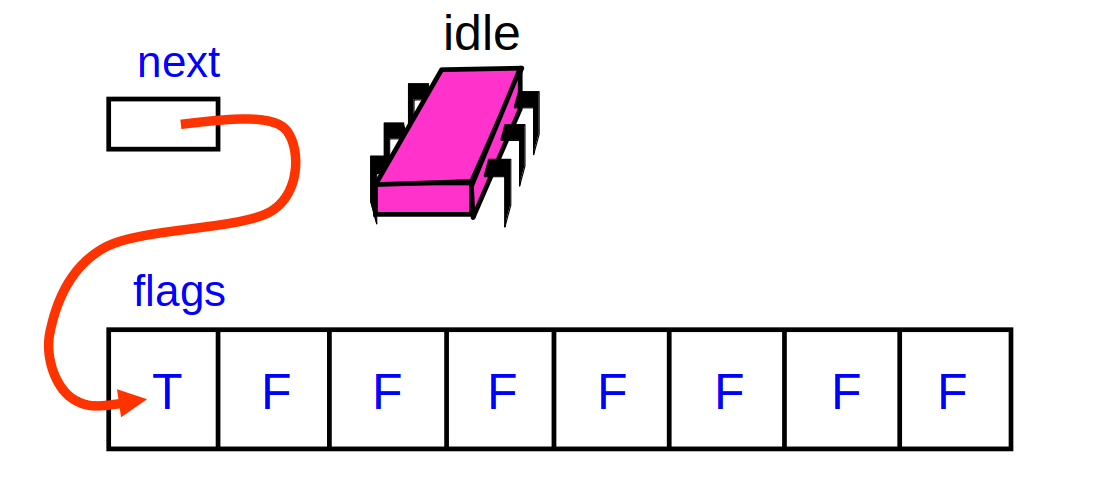
\includegraphics[width=0.7\textwidth]{./pics/alock/91.png} \end{center} }
\only<2>{ \begin{center} 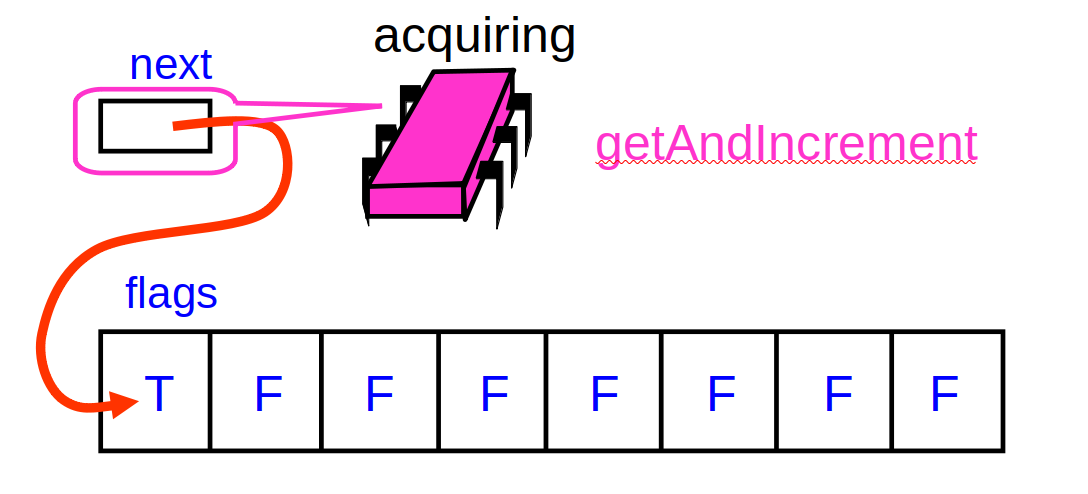
\includegraphics[width=0.7\textwidth]{./pics/alock/92.png} \end{center} }
\only<3>{ \begin{center} 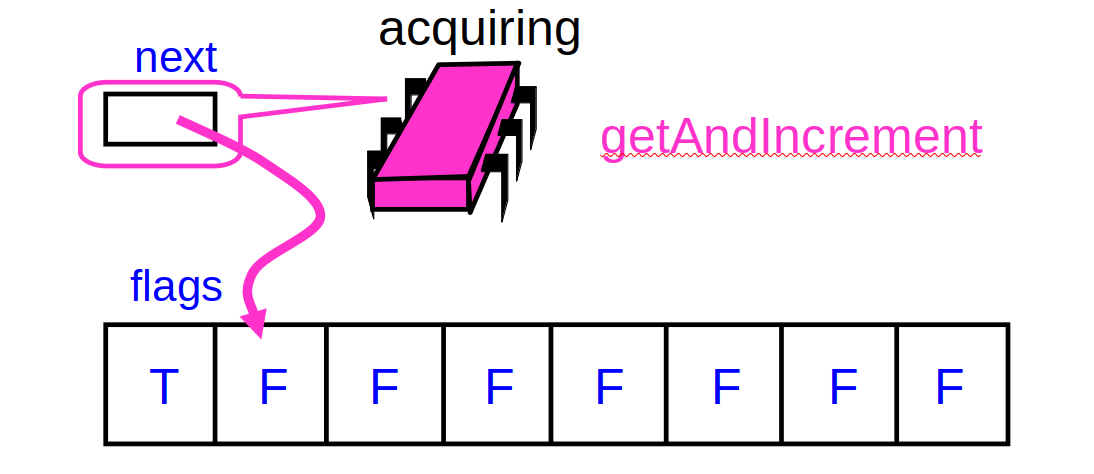
\includegraphics[width=0.7\textwidth]{./pics/alock/93.png} \end{center} }
\only<4>{ \begin{center} 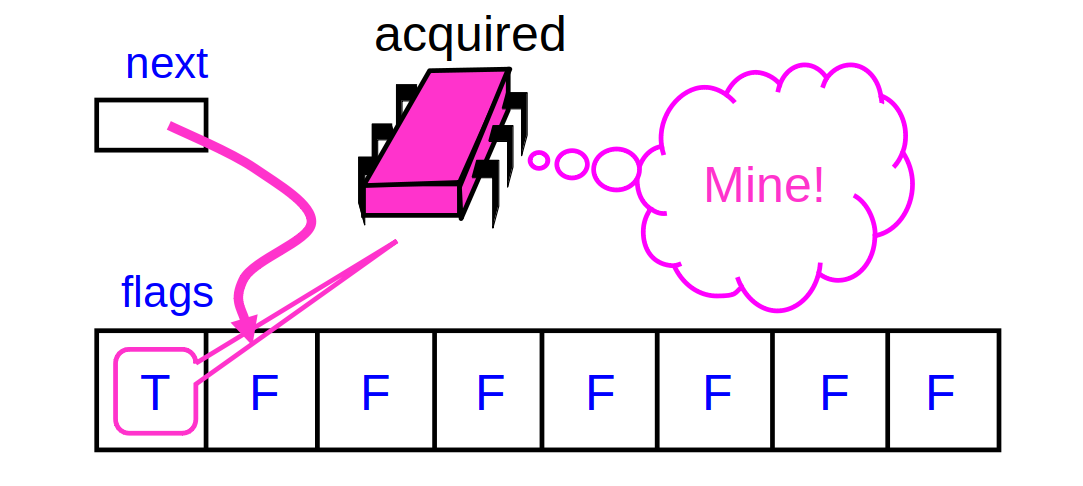
\includegraphics[width=0.7\textwidth]{./pics/alock/94.png} \end{center} }
\only<5>{ \begin{center} 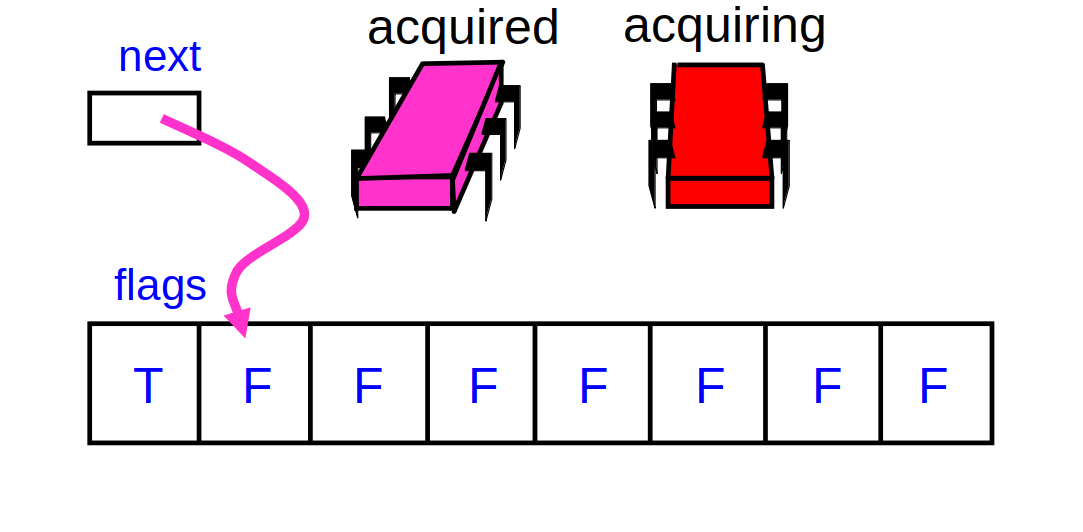
\includegraphics[width=0.7\textwidth]{./pics/alock/95.png} \end{center} }
\only<6>{ \begin{center} 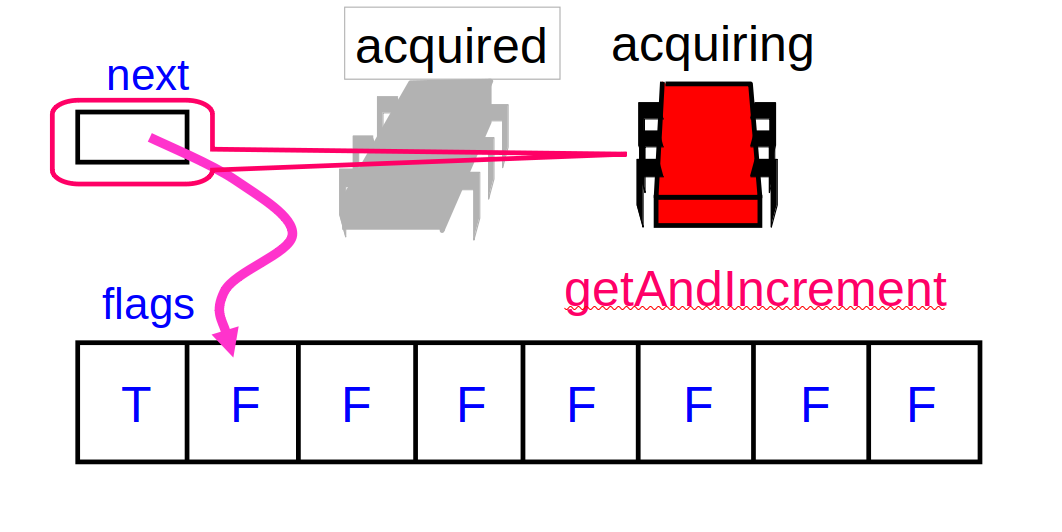
\includegraphics[width=0.7\textwidth]{./pics/alock/96.png} \end{center} }
\only<7>{ \begin{center} 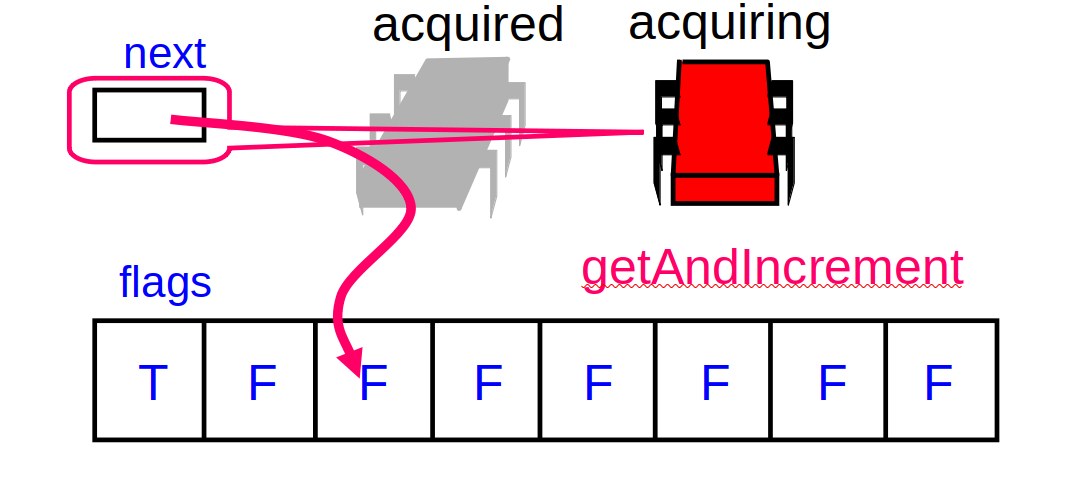
\includegraphics[width=0.7\textwidth]{./pics/alock/97.png} \end{center} }
\only<8>{ \begin{center} 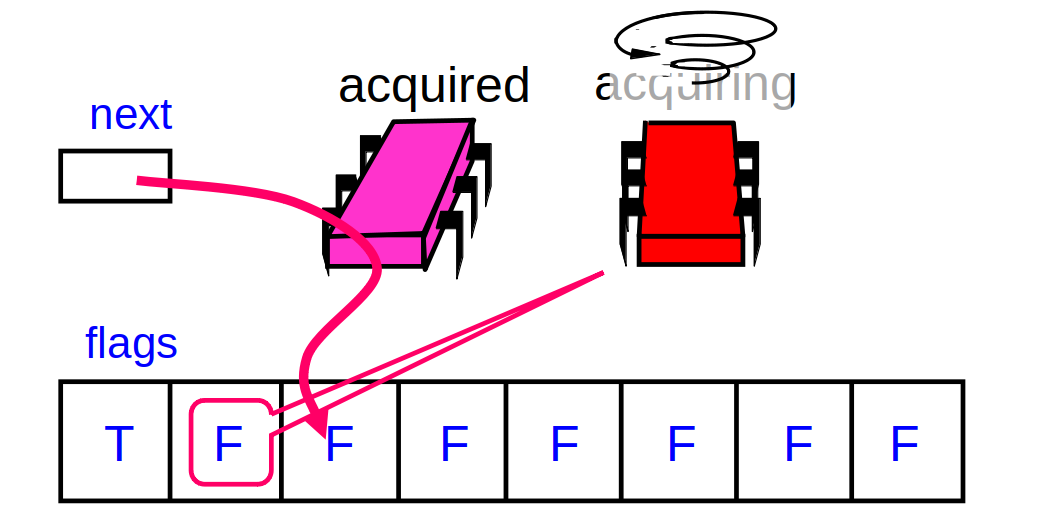
\includegraphics[width=0.7\textwidth]{./pics/alock/98.png} \end{center} }
\only<9>{ \begin{center} 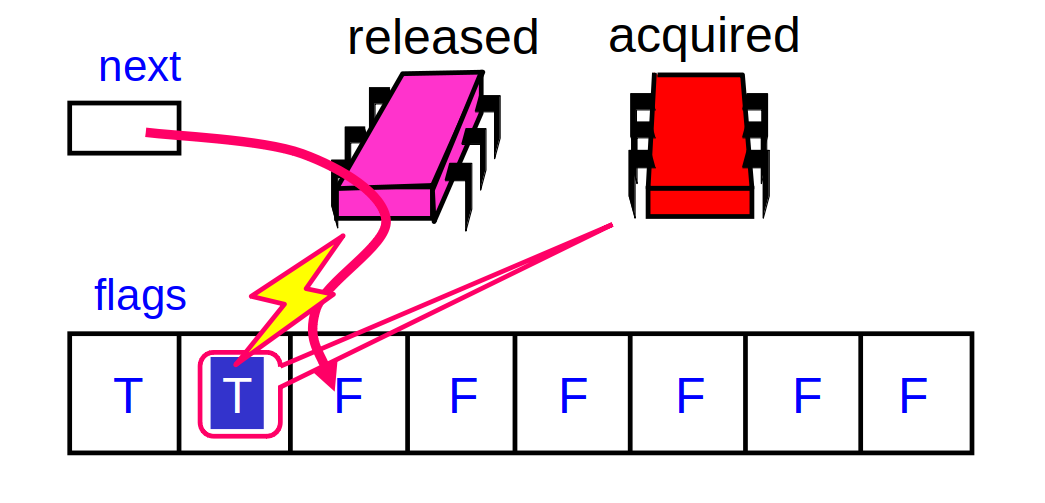
\includegraphics[width=0.7\textwidth]{./pics/alock/99.png} \end{center} }
\only<10>{ \begin{center} 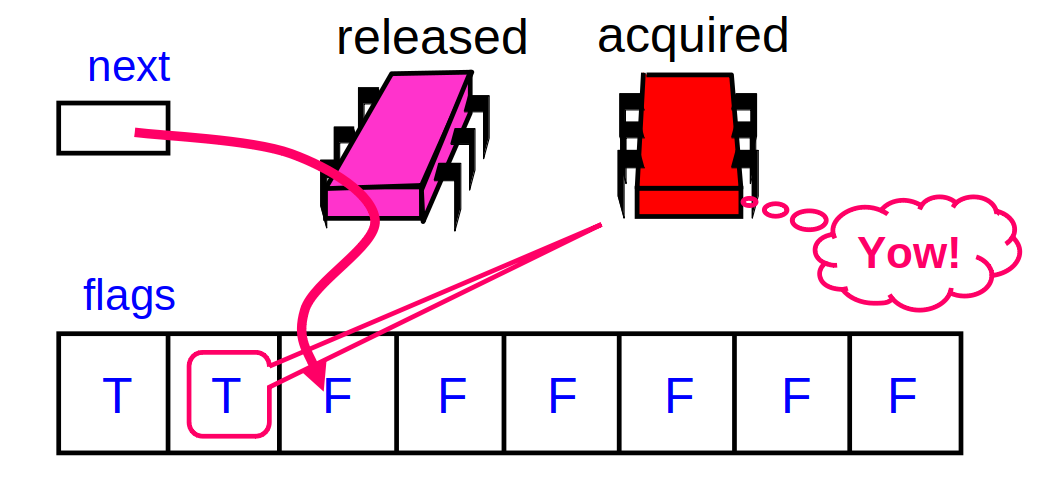
\includegraphics[width=0.7\textwidth]{./pics/alock/100.png} \end{center} }

\end{frame}

\begin{frame}[fragile]{Anderson Queue Lock}

\begin{minted}{java}
class ALock implements Lock {
  boolean[] flags = {true,false, ...,false}; // one flag per thread
  AtomicInteger next = new AtomicInteger(0); // next flag to use
  ThreadLocal<Integer> mySlot;               // thread-local variable
  public lock() {
    mySlot = next.getAndIncrement();         // take next slot
    while (flags[mySlot % n] == false) {};   // await
    flags[mySlot % n] = false;               // prepare slot for re-use
  }
  public unlock() {
    flags[(mySlot + 1) % n] = true;          // tell next thread to go
  }
\end{minted}

\end{frame}

\begin{frame}{False sharing}
\only<1>{ \begin{center} 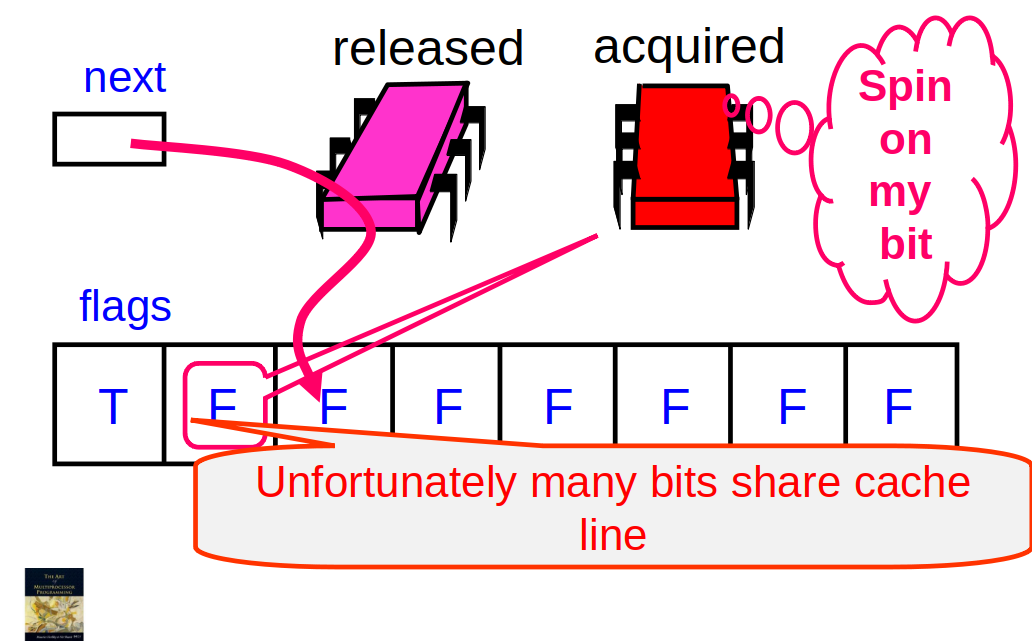
\includegraphics[width=0.7\textwidth]{./pics/alock/110.png} \end{center} }
\only<2>{ \begin{center} 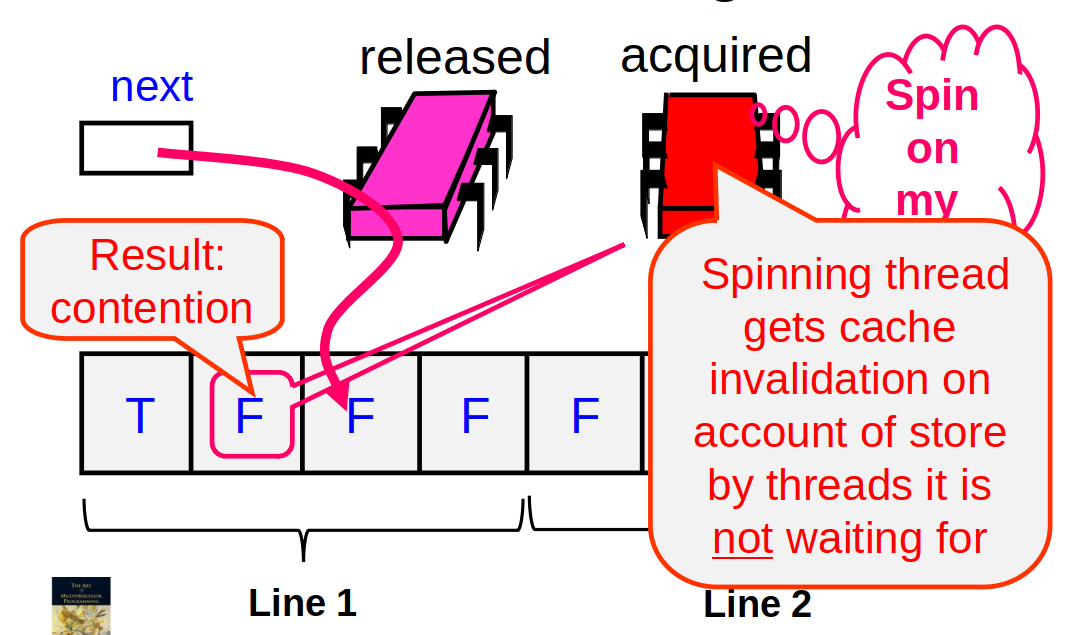
\includegraphics[width=0.7\textwidth]{./pics/alock/111.png} \end{center} }
\end{frame}

\begin{frame}{Solution: padding}
\only<1>{ \begin{center} 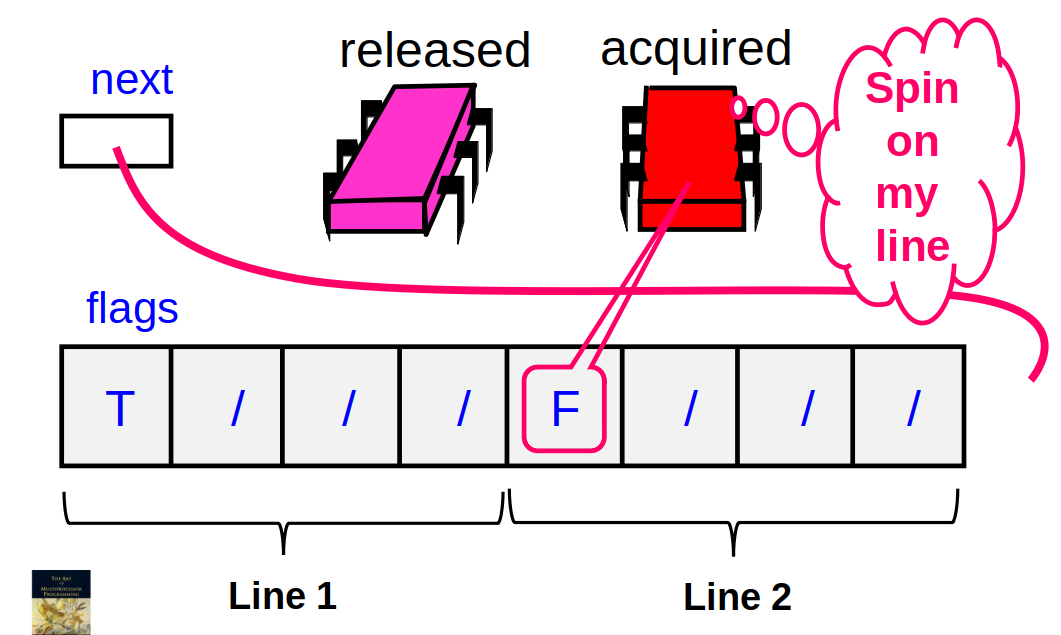
\includegraphics[width=0.7\textwidth]{./pics/alock/112.png} \end{center} }
\end{frame}

\begin{frame}{Anderson Queue Lock}

\textbf{Safety}
\begin{itemize}
  \item Mutual exclusion, Deadlock-freedom, Visibility
\end{itemize}

\textbf{Progress}
\begin{itemize}
  \item Starvation-freedom, \textbf{Fairness} (FIFO)
\end{itemize}

\textbf{Performance}
\begin{itemize}
  \item Memory overhead
  \begin{itemize}    
    \item cache line per competitor
    \item $O(LN)$ where $L$ = number of locks, $N$ = number of threads
    \item what if number of threads is unknown?   
  \end{itemize}
  \item Efficiency in contended mode, Scalability
  \begin{itemize}
    \item First "truly scalable"\ lock in our course
  \end{itemize}  
  \item Backoff policy  
  \begin{itemize}
    \item Spin me right round, baby, right round
  \end{itemize}  
\end{itemize}

\pause
\textbf{Idea:} use O(1) thread-local memory to decrease memory overhead

\end{frame}


\section{Queue-based locks: CLH}
\showTOC

\begin{frame}{CLH lock}

\begin{itemize}
  \item CLH -- Craig, Landin, Hagersten
  \item FIFO
  \item every thread has thread-private node to be used as a part of a queue
\end{itemize}  

\pause
We are discussing simplified implementation in Garbage-collected language (Java) to avoid manual memory management in concurrent environment

\pause
Reminder: in Lecture~\atomicsNum \ we broke lock-free stack by using node pooling (ABA problem)

\end{frame}


\begin{frame}{CLH lock: initialization}

\only<1>{ \begin{center} 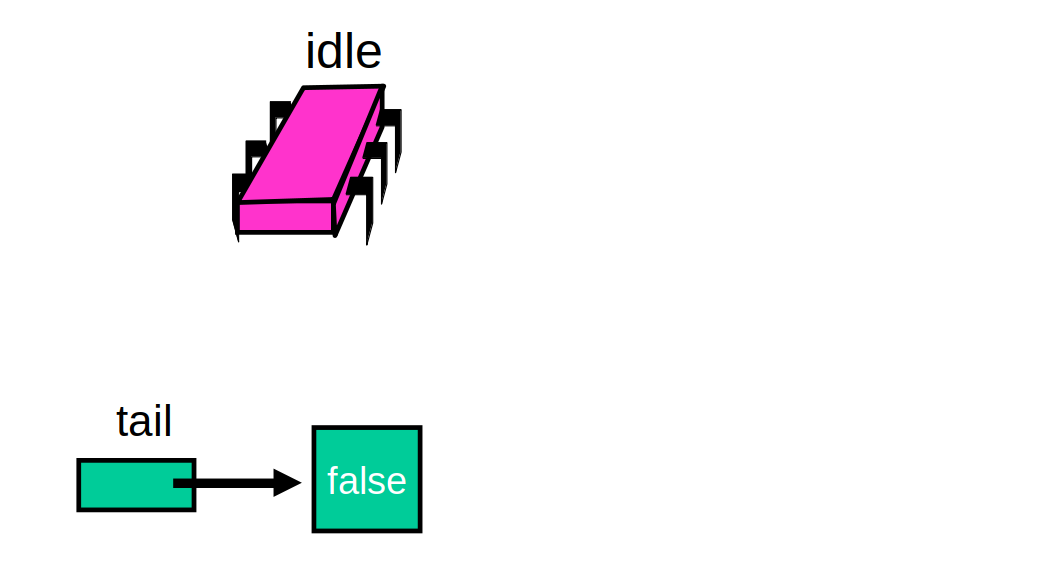
\includegraphics[width=0.7\textwidth]{./pics/clh/117.png} \end{center} }
\only<2>{ \begin{center} 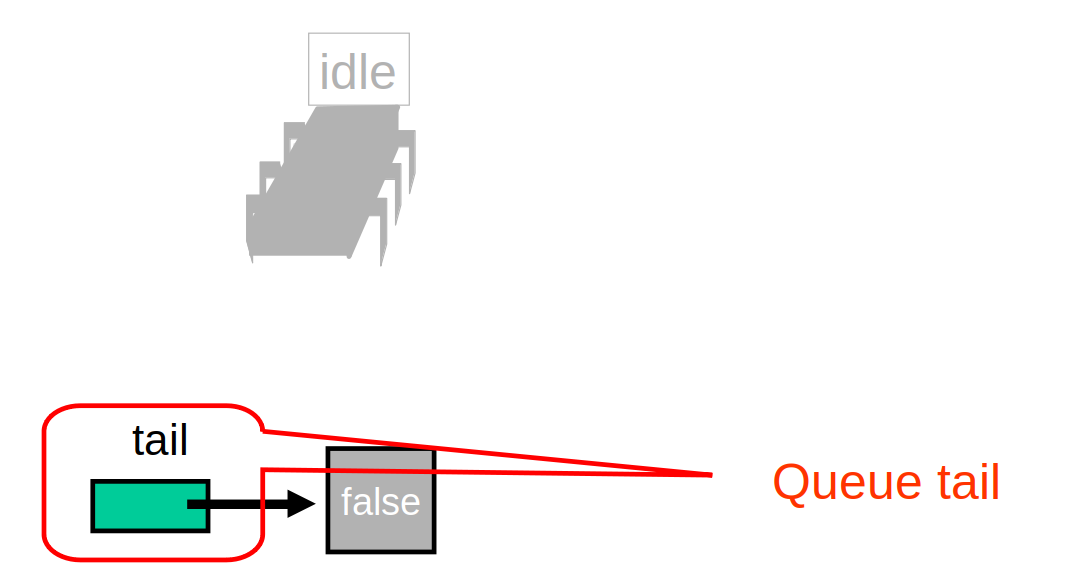
\includegraphics[width=0.7\textwidth]{./pics/clh/118.png} \end{center} }
\only<3>{ \begin{center} 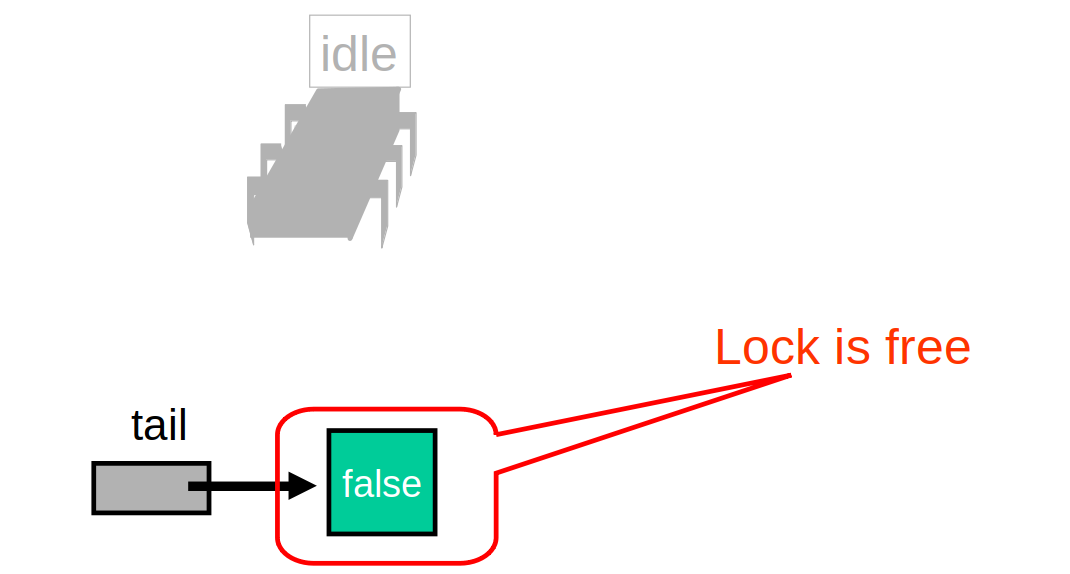
\includegraphics[width=0.7\textwidth]{./pics/clh/119.png} \end{center} }
\only<4>{ \begin{center} 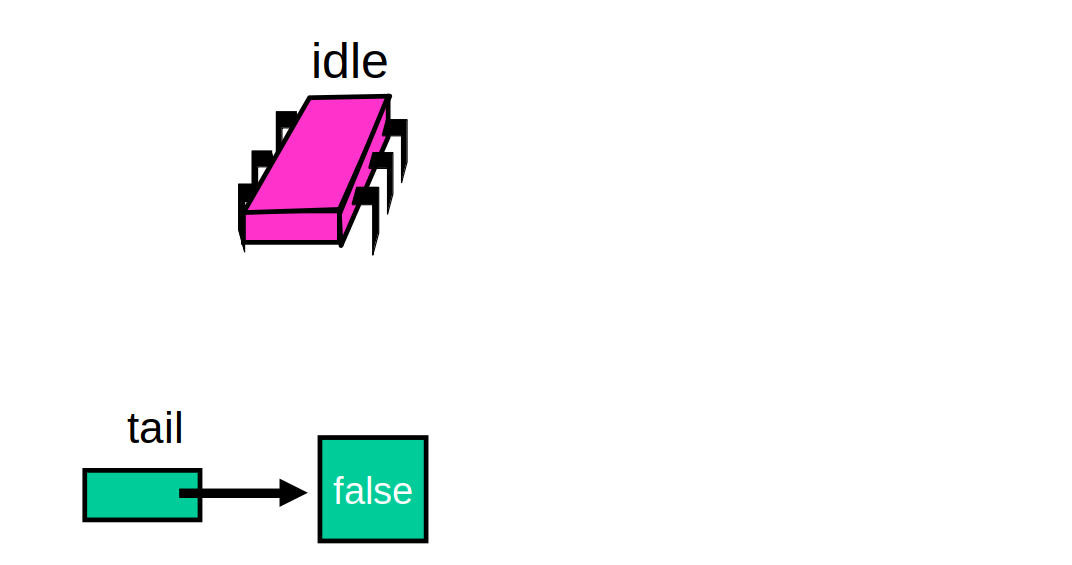
\includegraphics[width=0.7\textwidth]{./pics/clh/120.png} \end{center} }

\end{frame}

\begin{frame}[noframenumbering]{Purple Wants the Lock}
\only<1>{ \begin{center} 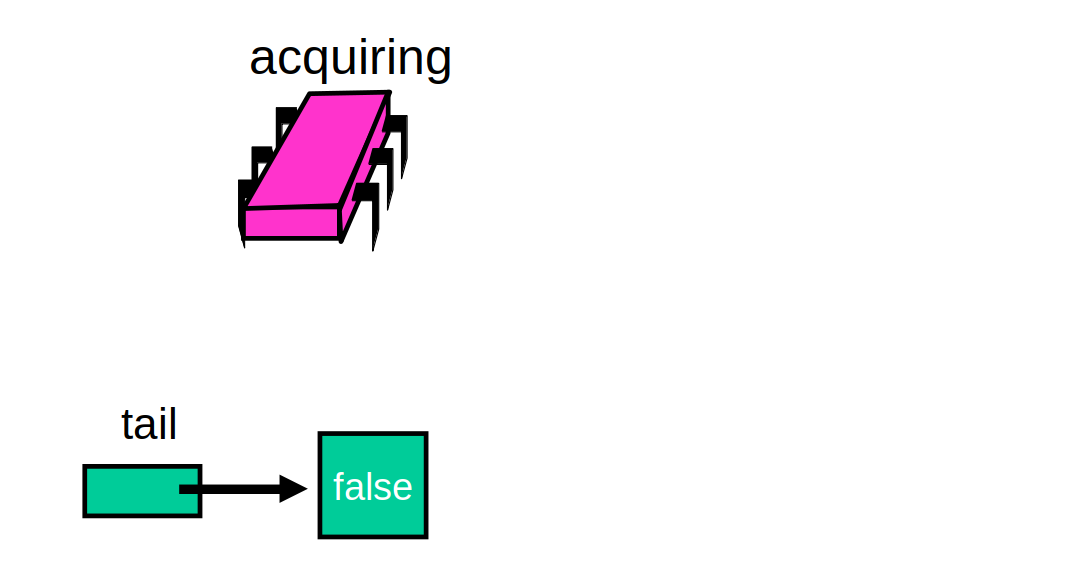
\includegraphics[width=0.7\textwidth]{./pics/clh/121.png} \end{center} }
\only<2>{ \begin{center} 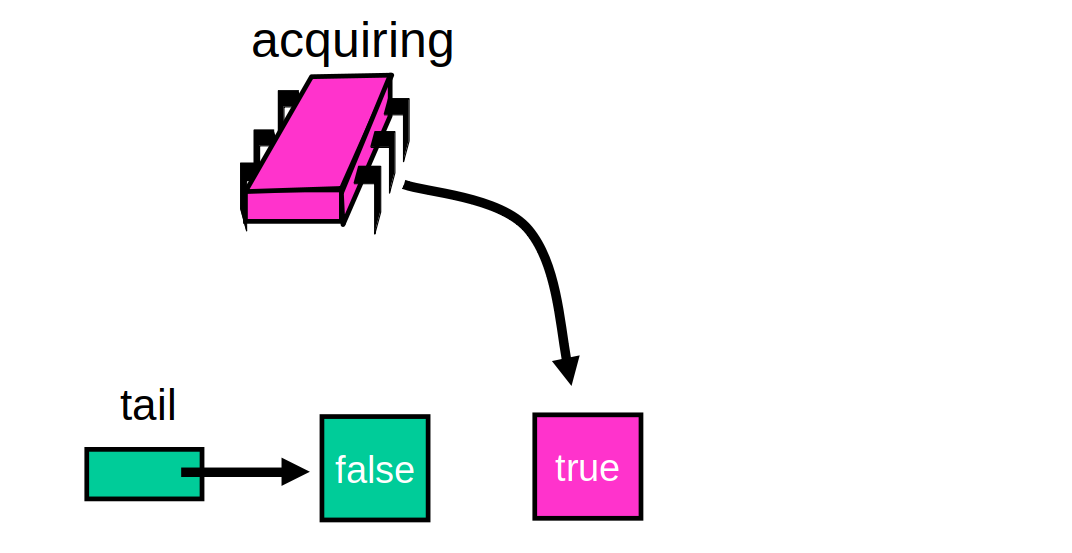
\includegraphics[width=0.7\textwidth]{./pics/clh/122.png} \end{center} }
\only<3>{ \begin{center} 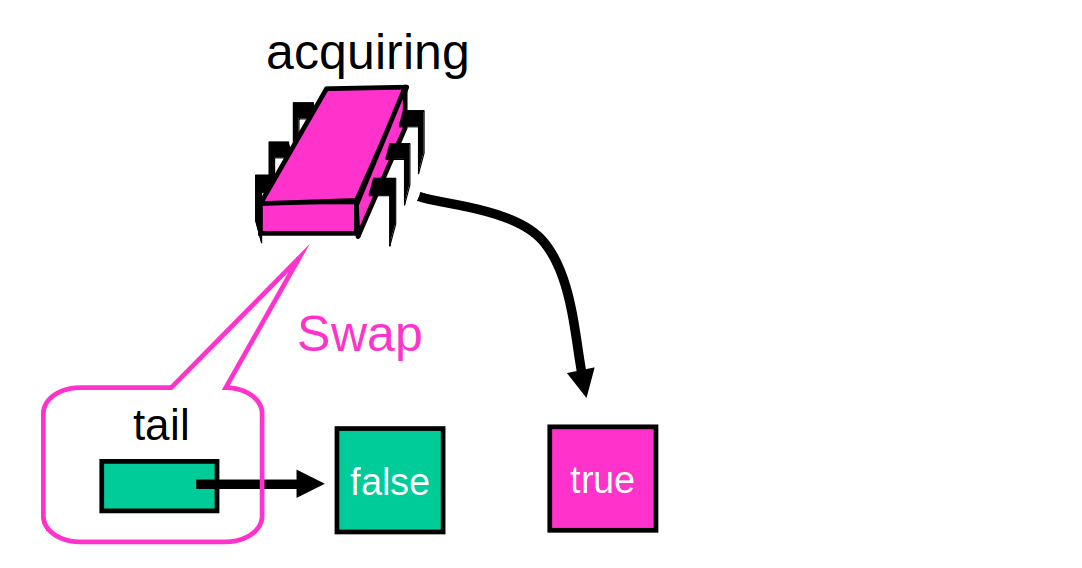
\includegraphics[width=0.7\textwidth]{./pics/clh/123.png} \end{center} }
\end{frame}

\begin{frame}[noframenumbering]{Purple Has the Lock}
\only<1>{ \begin{center} 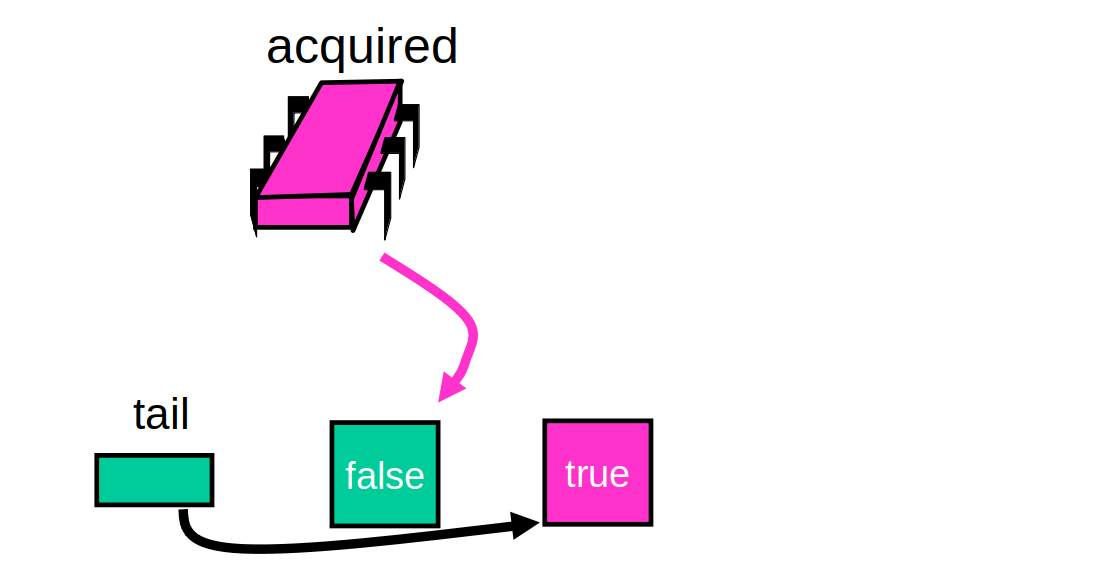
\includegraphics[width=0.7\textwidth]{./pics/clh/124.png} \end{center} }
\end{frame}

\begin{frame}[noframenumbering]{Red Wants the Lock}
\only<1>{ \begin{center} 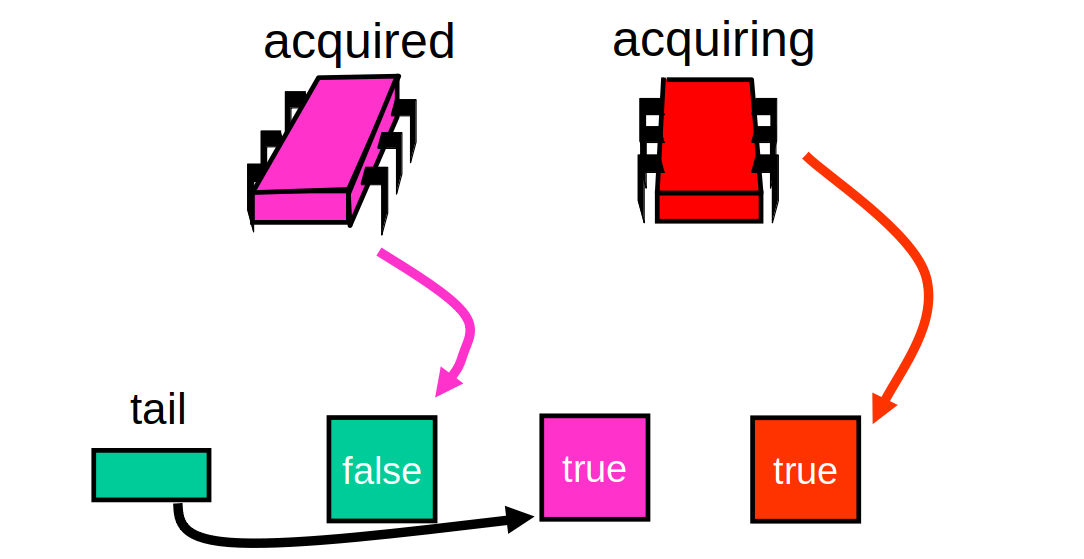
\includegraphics[width=0.7\textwidth]{./pics/clh/125.png} \end{center} }
\only<2>{ \begin{center} 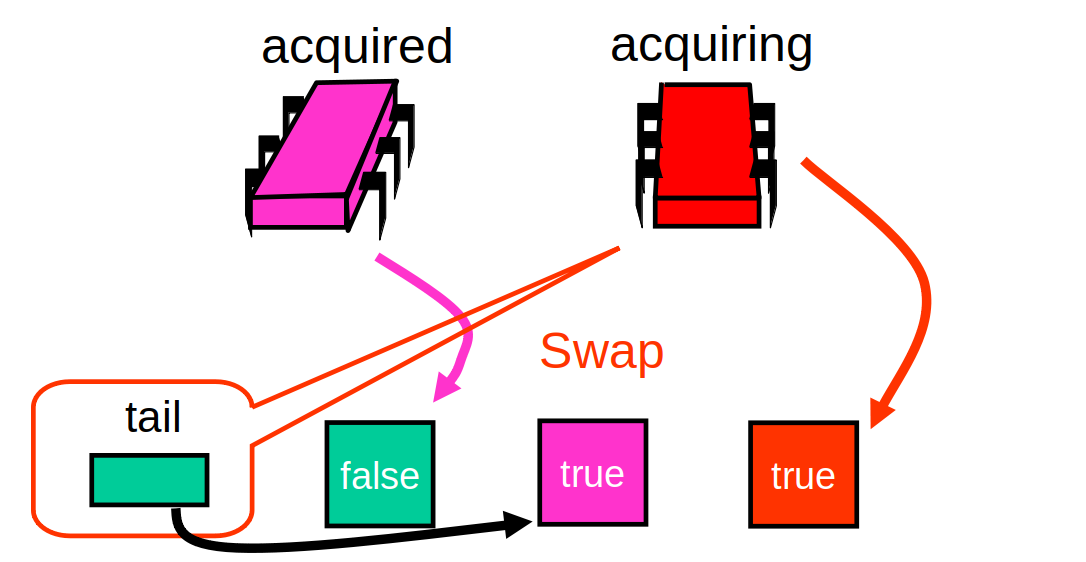
\includegraphics[width=0.7\textwidth]{./pics/clh/126.png} \end{center} }
\only<3>{ \begin{center} 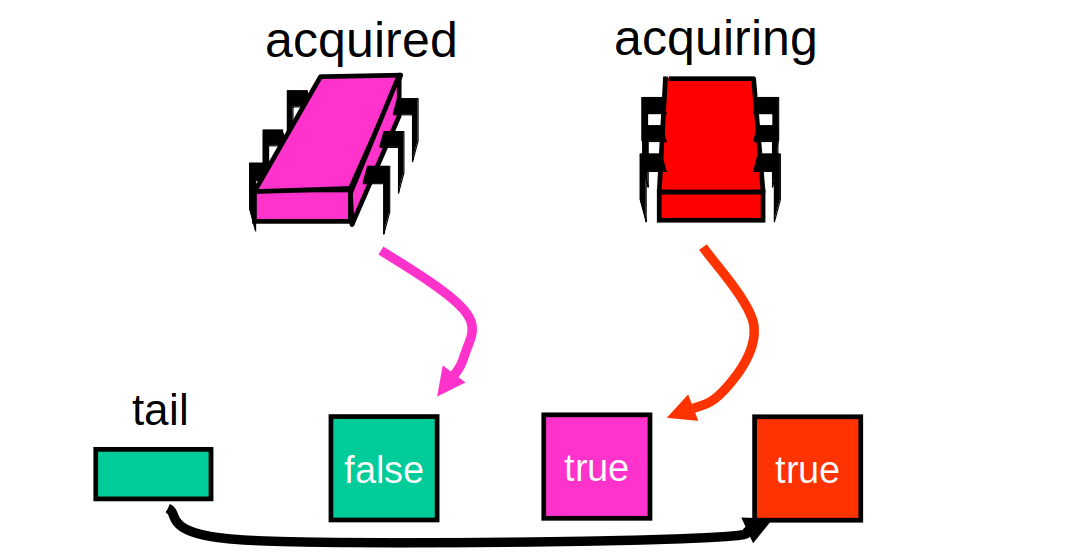
\includegraphics[width=0.7\textwidth]{./pics/clh/127.png} \end{center} }
\only<4>{ \begin{center} 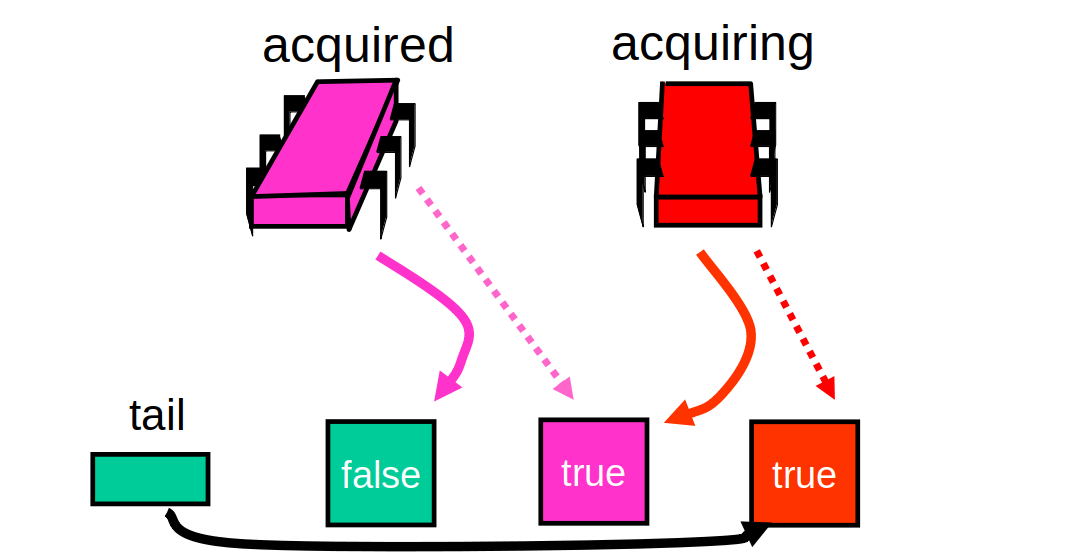
\includegraphics[width=0.7\textwidth]{./pics/clh/128.png} \end{center} }
\only<5>{ \begin{center} 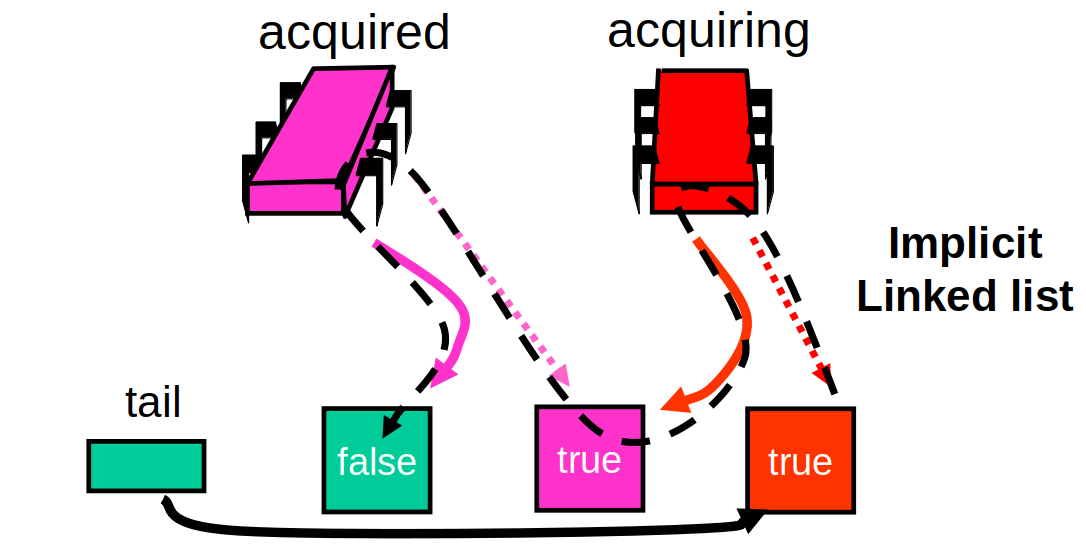
\includegraphics[width=0.7\textwidth]{./pics/clh/129.png} \end{center} }
\only<6>{ \begin{center} 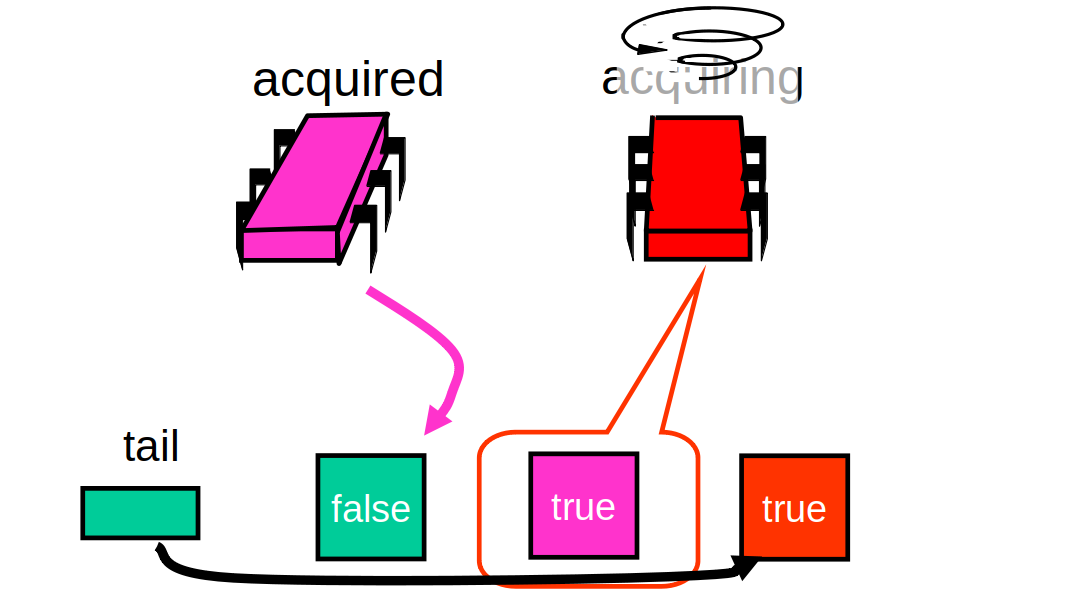
\includegraphics[width=0.7\textwidth]{./pics/clh/130.png} \end{center} }
\only<7>{ \begin{center} 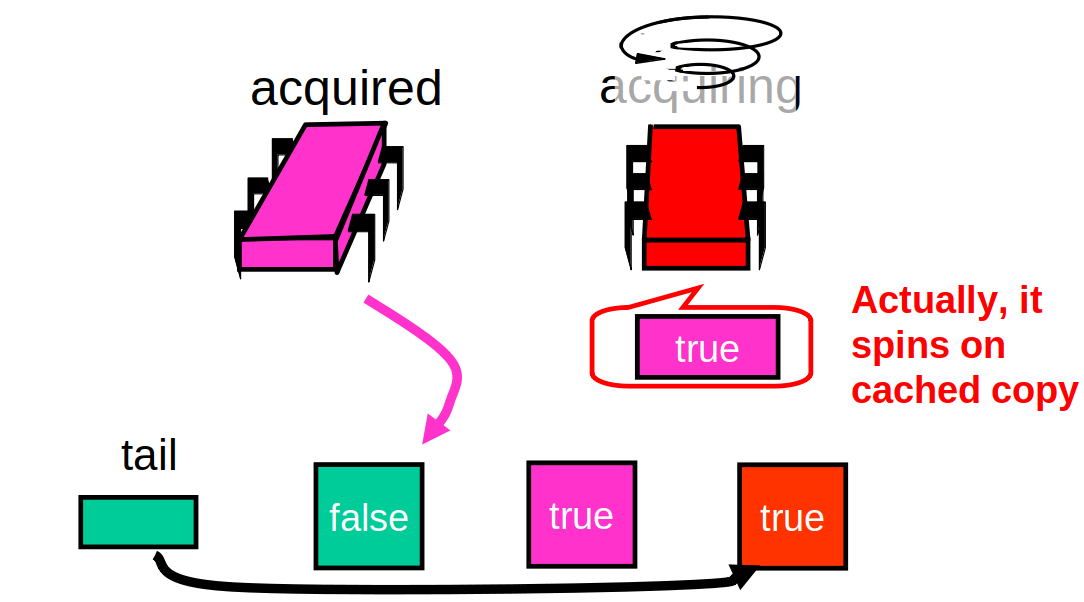
\includegraphics[width=0.7\textwidth]{./pics/clh/131.png} \end{center} }
\end{frame}

\begin{frame}[noframenumbering]{Purple Releases}
\only<1>{ \begin{center} 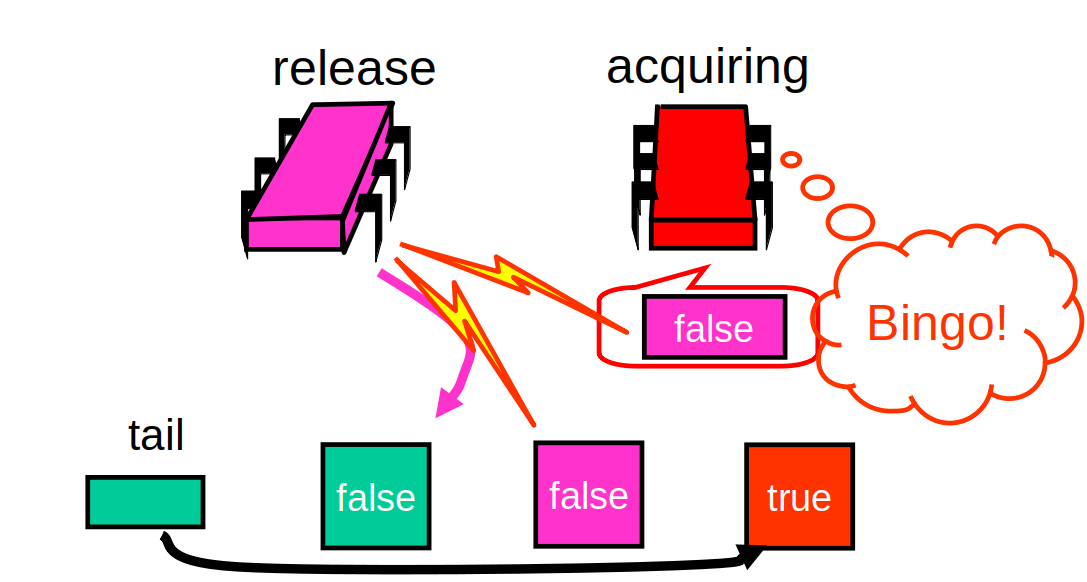
\includegraphics[width=0.7\textwidth]{./pics/clh/132.png} \end{center} }
\only<2>{ \begin{center} 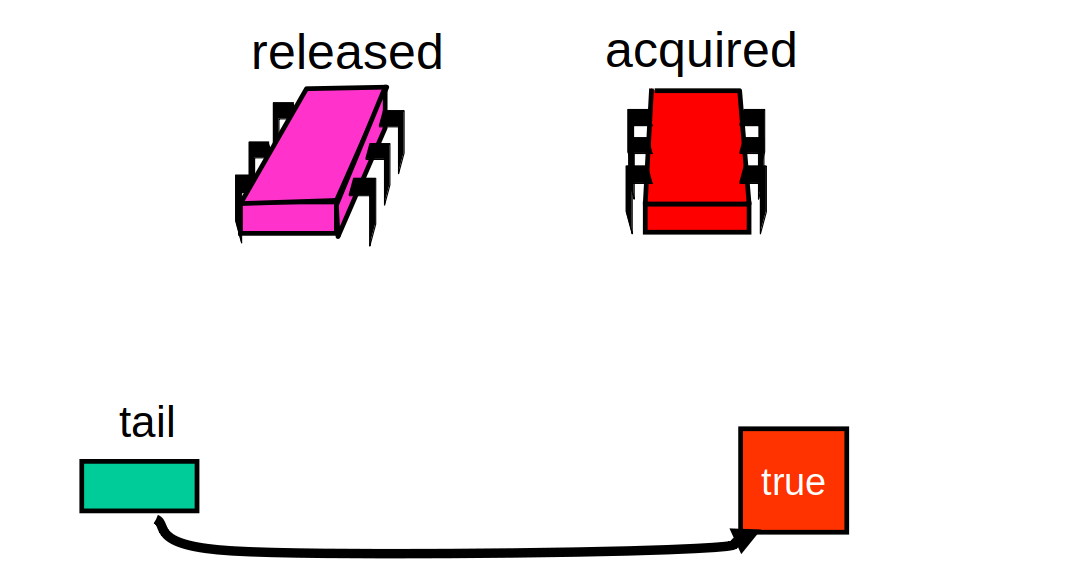
\includegraphics[width=0.7\textwidth]{./pics/clh/133.png} \end{center} }
\end{frame}

\begin{frame}[fragile]{CLH}
\begin{minted}{java}
class Qnode { AtomicBoolean locked = new AtomicBoolean(); }
class CLHLock implements Lock {
  AtomicReference<Qnode> tail = new AtomicReference(new Qnode(false));
  ThreadLocal<Qnode> node;     // thread-local variable
  public void lock() {
    node.set(new Qnode(true)); // allocate my node as not released
    Qnode pred = tail.getAndSet(node.get()); // swap in my node
    while (pred.locked.get()) {} // spin until predecessor releases lock
  }
  public void unlock() {
    node.get().locked.set(false); // notify successor
    node.set(null);            // node is not needed by current thread
                               // but could still be read by other threads
                               // cannot `free` it
  }
\end{minted}
\end{frame}

\begin{frame}{CLH: summary}

\textbf{Safety}
\begin{itemize}
  \item Mutual exclusion, Deadlock-freedom, Visibility
\end{itemize}

\textbf{Progress}
\begin{itemize}
  \item Starvation-freedom, \textbf{Fairness} (FIFO)
\end{itemize}

\textbf{Performance}
\begin{itemize}
  \item Memory overhead
  \begin{itemize}
    \item fixed-size node per competitor
    \item $O(L+N)$ where $L$ = number of locks, $N$ = number of threads
  \end{itemize}
  \item Efficiency in contended mode, Scalability
  \begin{itemize}
    \item Second "truly scalable"\ lock in our course
    \item Spins on random \textbf{remote} memory location
  \end{itemize}  
  \item Backoff policy  
  \begin{itemize}
    \item Spin me right round, baby, right round
  \end{itemize}  
\end{itemize}
\end{frame}


\begin{frame}[t]{CLH: locality}

Contender of CLH lock spins on random \textbf{remote} memory location

\pause


NUMA Architectures:
\begin{itemize}
  \item \textbf{N}on-\textbf{U}niform \textbf{M}emory \textbf{A}rchitecture
  \item Illusion: flat shared memory
  \item Truth: 
  \begin{itemize}
    \item No caches (sometimes)
    \item Some memory regions faster than others
  \end{itemize}
\end{itemize}

\end{frame}

\begin{frame}[fragile,t]{NUMA and locking}

Contender of CLH lock spins on random \textbf{remote} memory location

\begin{tabular}{cc}
\begin{center} 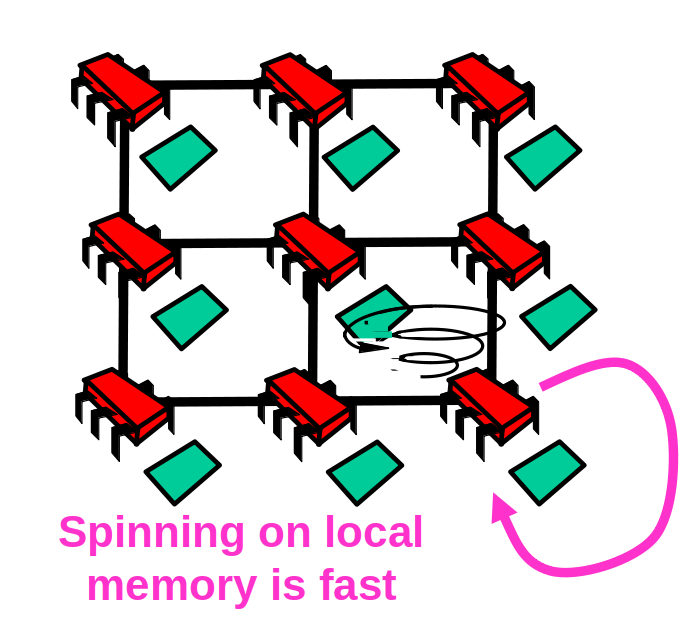
\includegraphics[width=0.4\textwidth]{./pics/numa/148.png} \end{center} 
&
\begin{center} 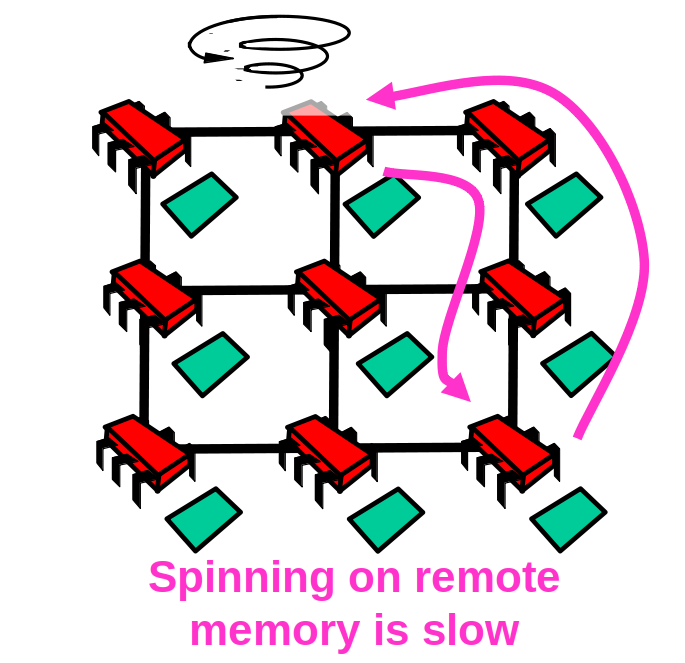
\includegraphics[width=0.4\textwidth]{./pics/numa/149.png} \end{center} 
\end{tabular}

\end{frame}

\begin{frame}[fragile,t,noframenumbering]{NUMA and locking}

Contender of CLH lock spins on random \textbf{remote} memory location

\textbf{Idea:} spin on thread-private memory

\begin{tabular}{cc}
\begin{center} 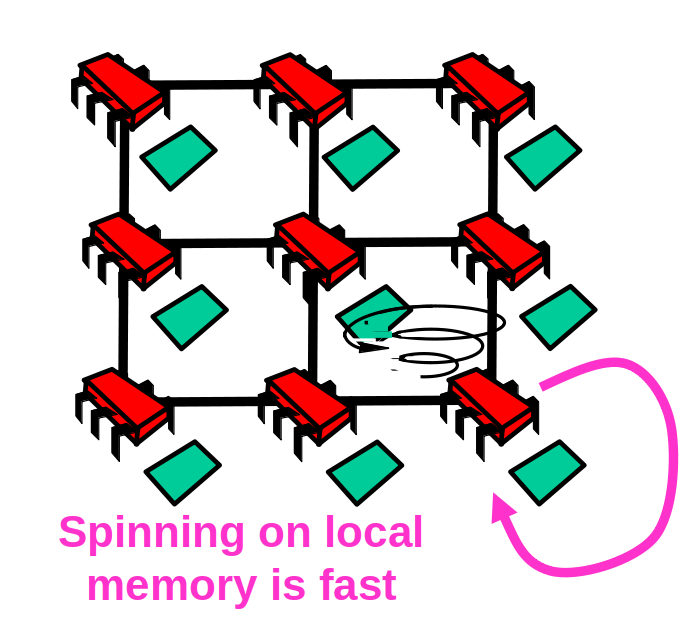
\includegraphics[width=0.4\textwidth]{./pics/numa/148.png} \end{center} 
&
\begin{center} 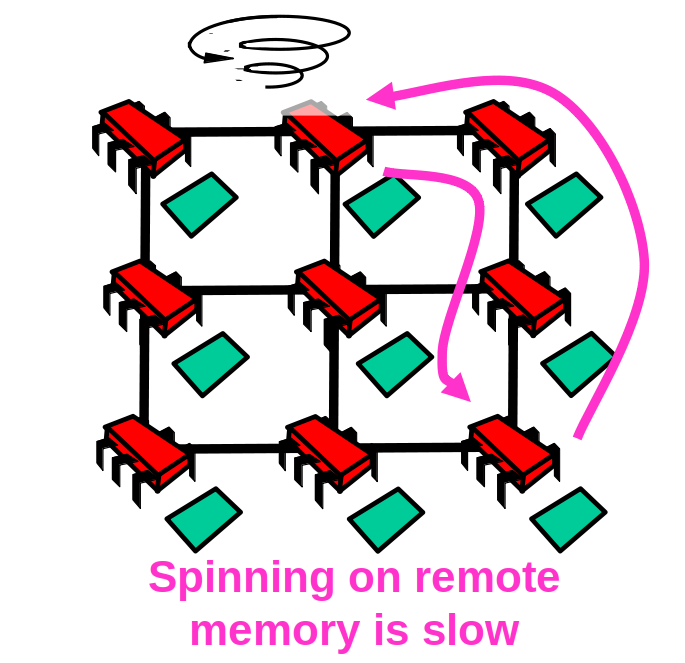
\includegraphics[width=0.4\textwidth]{./pics/numa/149.png} \end{center} 
\end{tabular}
\end{frame}

\section{Queue-based locks: MCS}
\showTOC

\begin{frame}{MCS}

\begin{itemize}
  \item MCS -- Mellor-Crummey and Scott
  \item FIFO
  \item every thread has thread-private node to be used as a part of a queue
  \item thread spins on this thread-local memory
\end{itemize}  

\pause
We are discussing simplified implementation in Garbage-collected language (Java) to avoid manual memory management in concurrent environment

\pause
Reminder: in Lecture~\atomicsNum \ we broke lock-free stack by using node pooling (ABA problem)
\end{frame}

\begin{frame}{MCS lock: initialization}
\only<1>{ \begin{center} 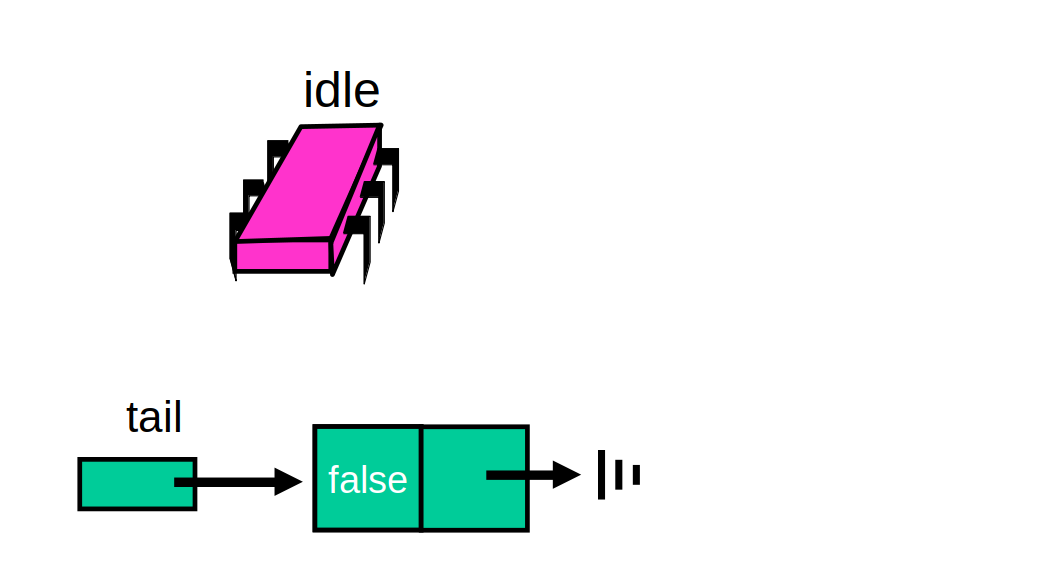
\includegraphics[width=0.7\textwidth]{./pics/mcs/152.png} \end{center} }
\end{frame}

\begin{frame}[noframenumbering]{Acquiring}
\only<1>{ \begin{center} 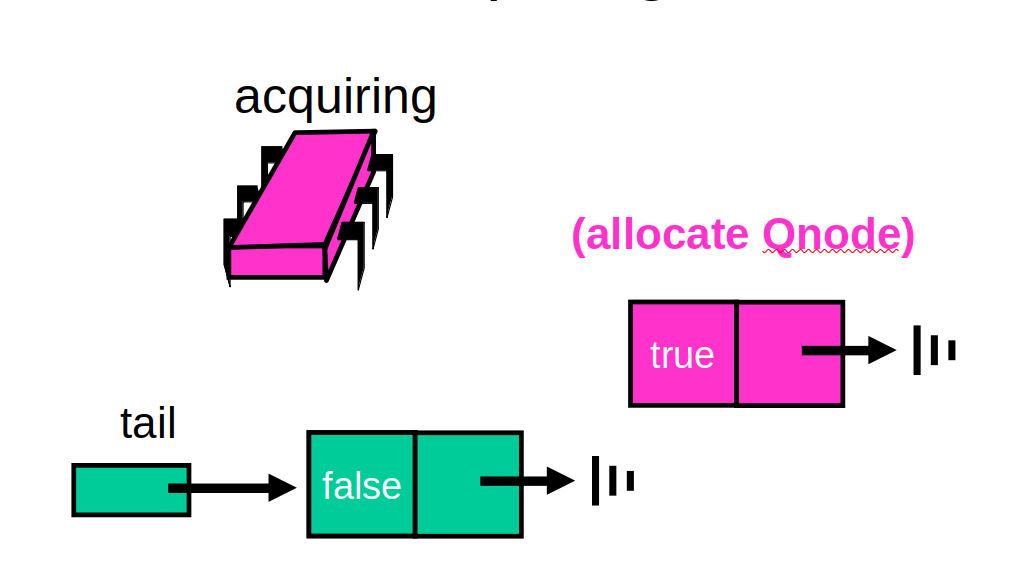
\includegraphics[width=0.7\textwidth]{./pics/mcs/153.png} \end{center} }
\only<2>{ \begin{center} 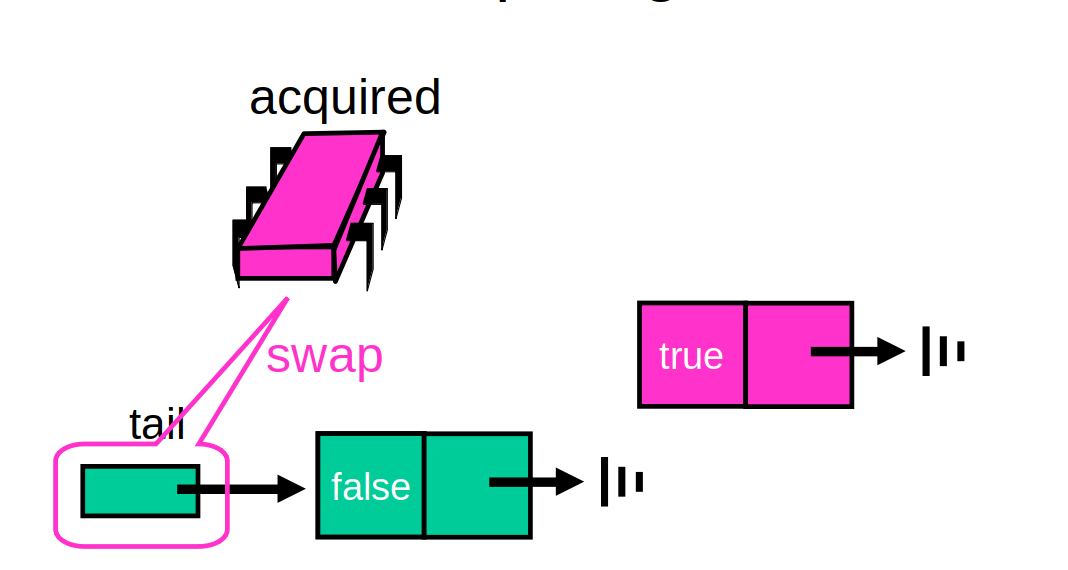
\includegraphics[width=0.7\textwidth]{./pics/mcs/154.png} \end{center} }
\only<3>{ \begin{center} 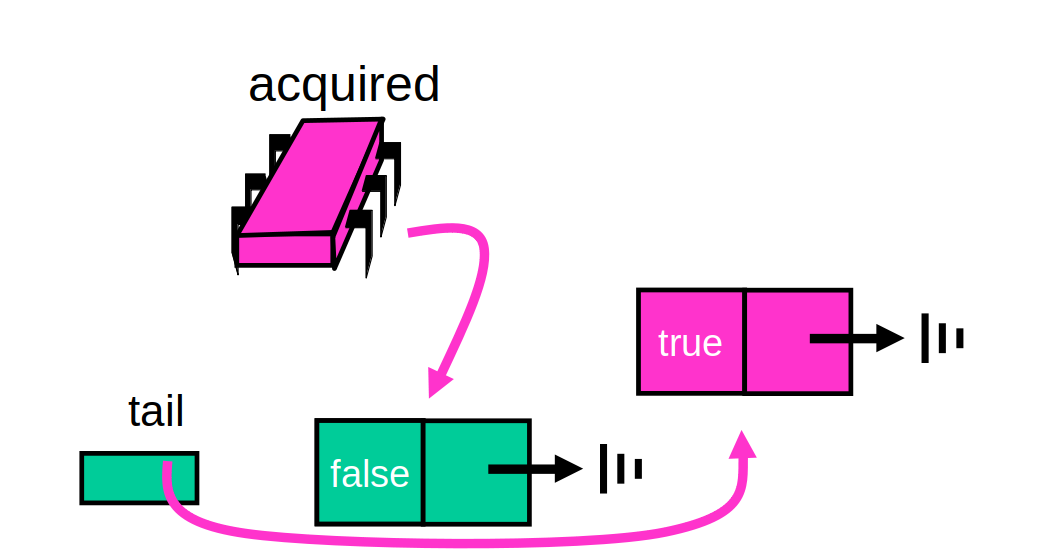
\includegraphics[width=0.7\textwidth]{./pics/mcs/155.png} \end{center} }
\end{frame}

\begin{frame}[noframenumbering]{Acquired}
\only<1>{ \begin{center} 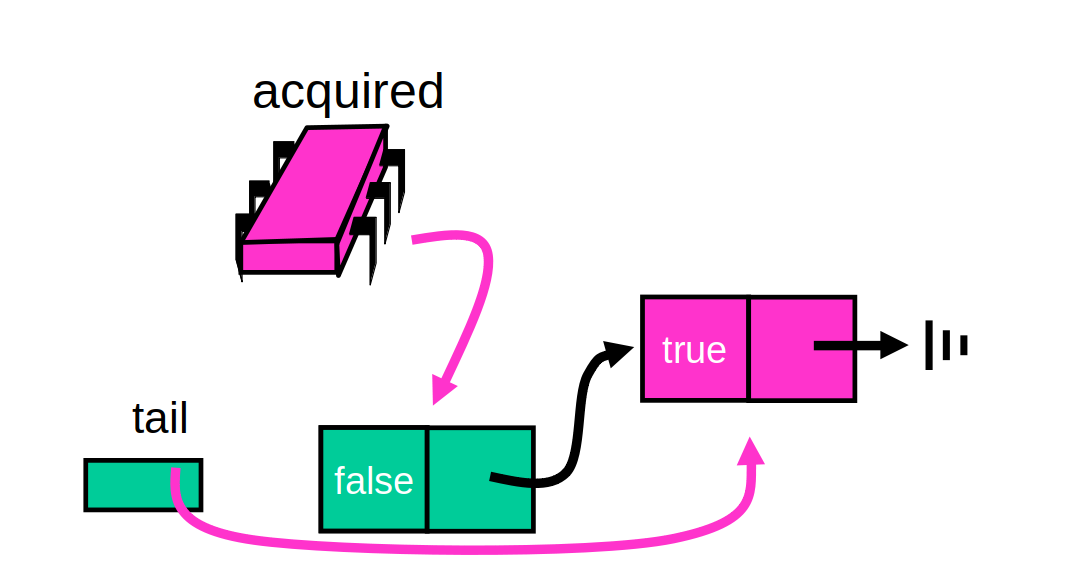
\includegraphics[width=0.7\textwidth]{./pics/mcs/156.png} \end{center} }
\end{frame}

\begin{frame}[noframenumbering]{Acquiring}
\only<1>{ \begin{center} 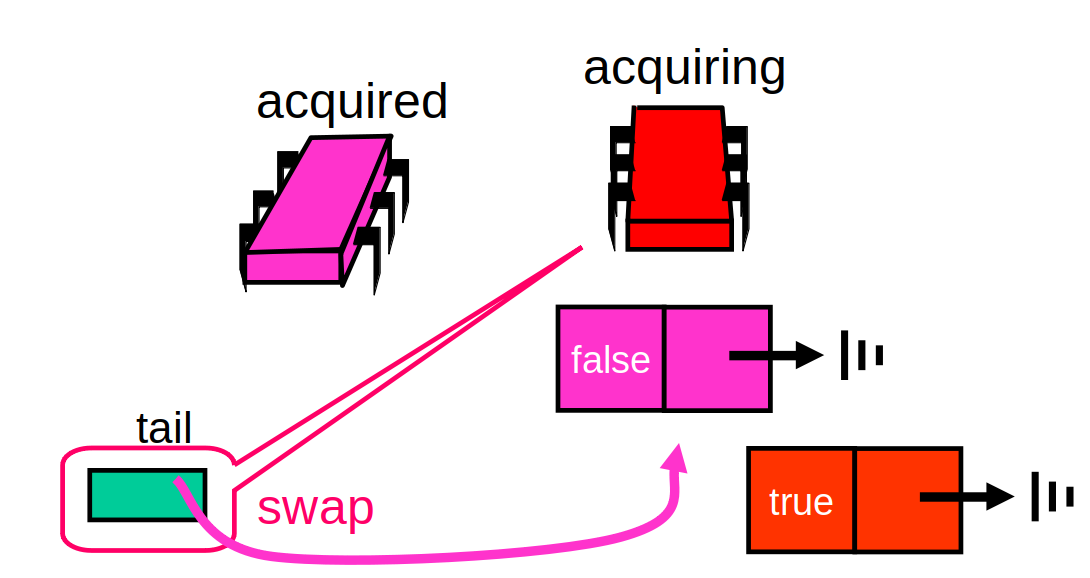
\includegraphics[width=0.7\textwidth]{./pics/mcs/157.png} \end{center} }
\only<2>{ \begin{center} 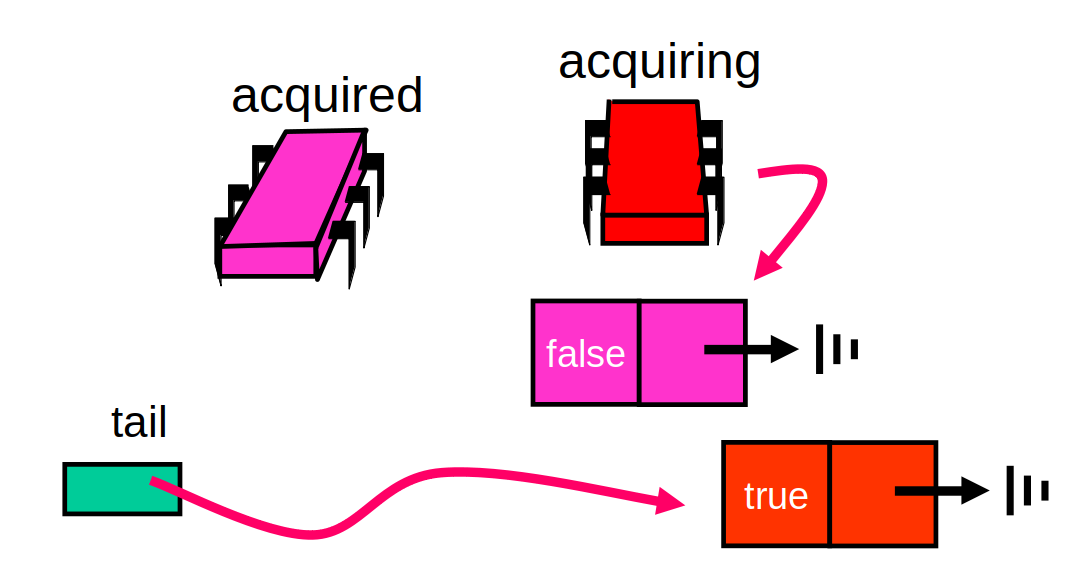
\includegraphics[width=0.7\textwidth]{./pics/mcs/158.png} \end{center} }
\only<3>{ \begin{center} 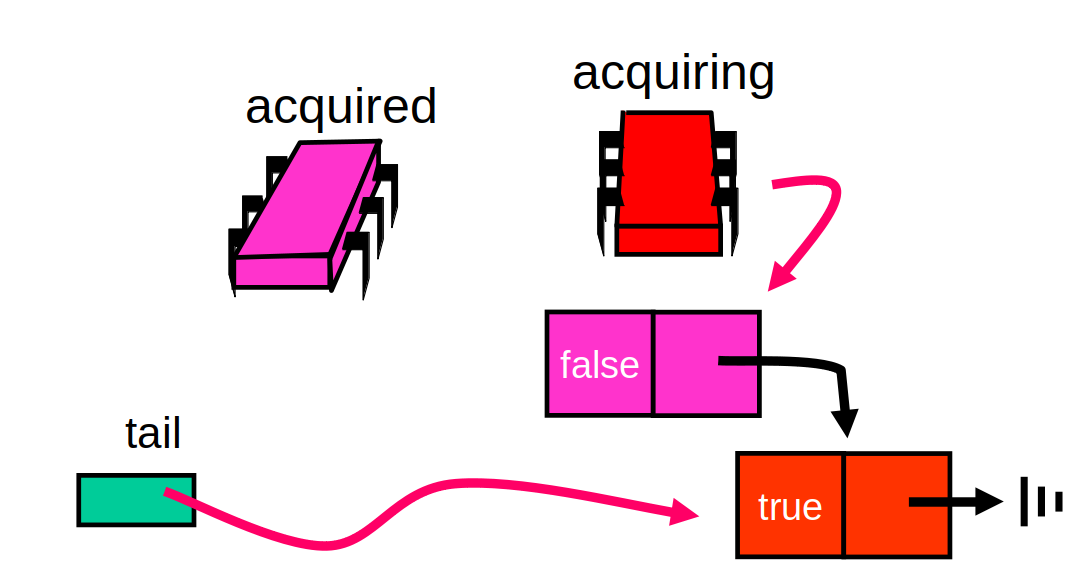
\includegraphics[width=0.7\textwidth]{./pics/mcs/159.png} \end{center} }
\only<4>{ \begin{center} 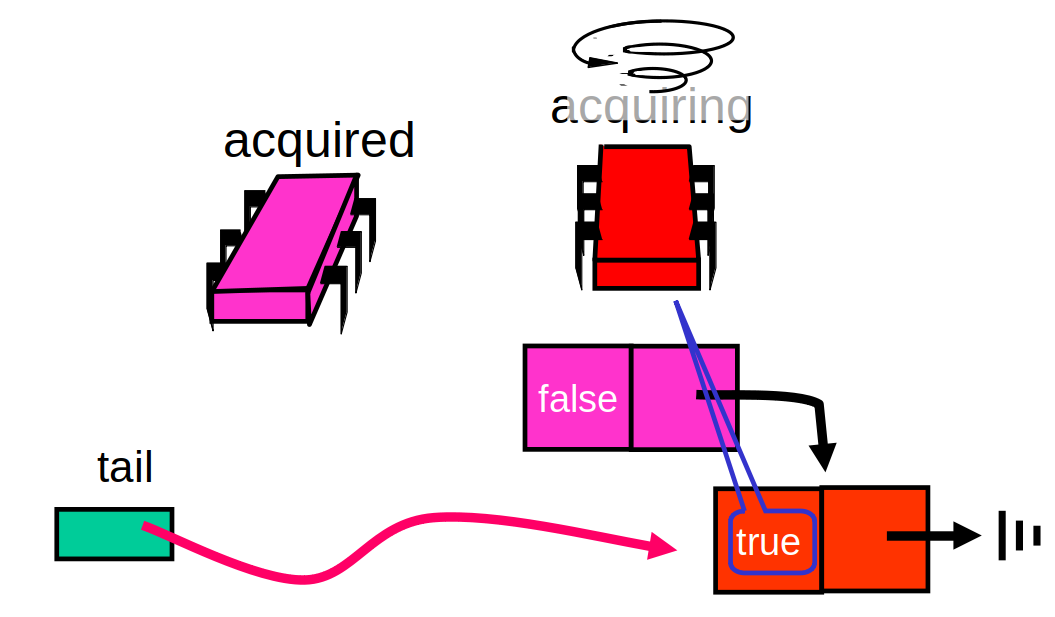
\includegraphics[width=0.7\textwidth]{./pics/mcs/160.png} \end{center} }
\only<5>{ \begin{center} 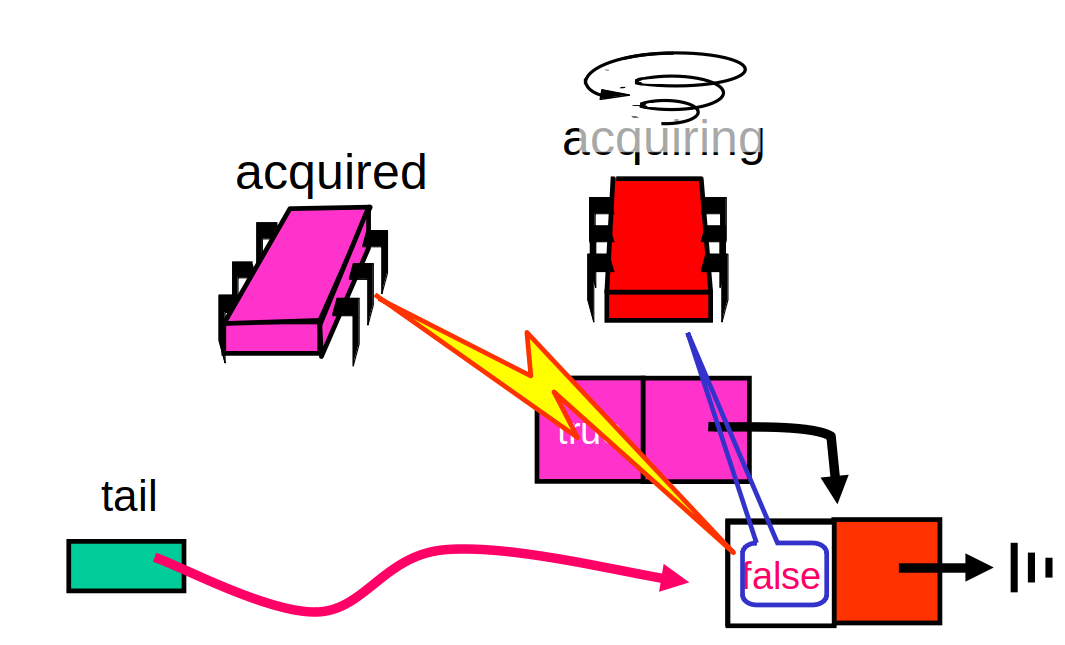
\includegraphics[width=0.7\textwidth]{./pics/mcs/161.png} \end{center} }
\only<6>{ \begin{center} 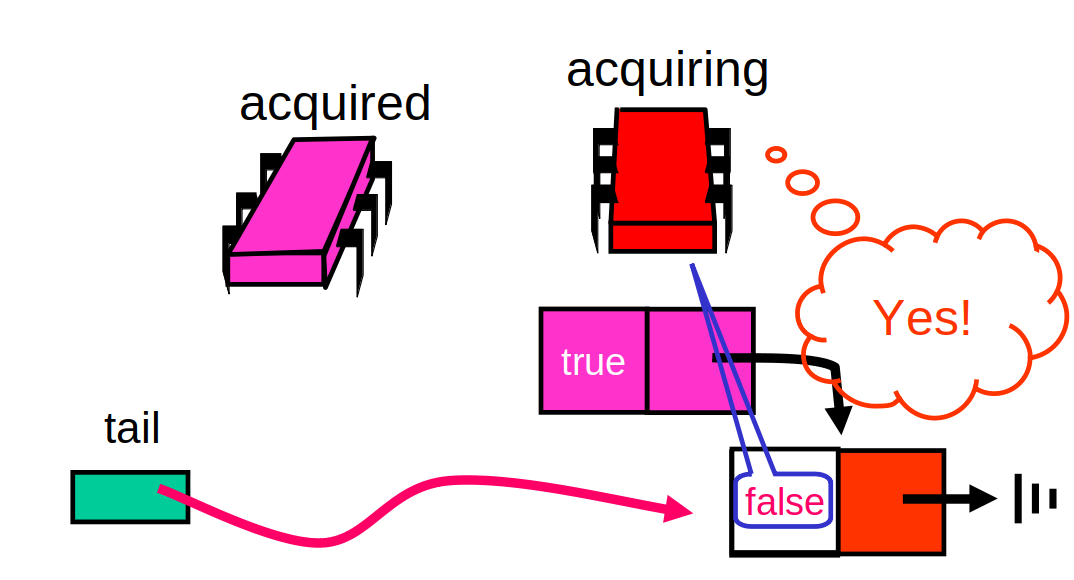
\includegraphics[width=0.7\textwidth]{./pics/mcs/162.png} \end{center} }
\end{frame}

\begin{frame}[t,fragile]{MCS: definitions}
\begin{minted}{java}
class Qnode { 
  AtomicBoolean locked = new AtomicBoolean(false); 
  AtomicReference<Qnode> next = new AtomicReference<Qnode>(null); 
}
Qnode qnode, pred;
// shortcut: boolean assignment
  qnode.locked = true;   // pseudocode
  qnode.locked.set(true) // java code
// shortcut: reference assignment
  pred.next = qnode;     // pseudocode
  pred.next.set(qnode)   // java code
\end{minted}
\end{frame}

\begin{frame}[t,fragile]{MCS: definitions}
\begin{minted}{java}
class Qnode {  var locked = new AtomicBoolean(false); 
               var next = new AtomicReference<Qnode>(null); }
ThreadLocal<Qnode> node = ...
Qnode qnode, pred;
// shortcut: init thread locals
  node = new Qnode(...);    // pseudocode
  node.set(new Qnode(...)); // java code
// shortcut: use thread locals
  pred.next = node;          // pseudocode
  pred.next.set(node.get()); // java code
\end{minted}
\end{frame}


\begin{frame}[t,fragile]{MCS: lock}
\begin{minted}{java}
class MCSLock implements Lock {
  AtomicReference<Qnode> tail = new AtomicReference<>(null);
  ThreadLocal<Qnode> node; // thread-local variable
  public void lock() {
    node = new Qnode(locked = false, next = null);    
    Qnode pred = tail.getAndSet(node); // swap in my node
    if (pred != null) { // fix if queue was non-empty
      node.locked = true;
      pred.next = node; // now other thread could see my node 
      while (node.locked) {} // wait until unlocked
    }
  }
}
\end{minted}
\end{frame}


\begin{frame}[t,fragile]{MCS: unlock}
\begin{minted}{java}
class MCSLock implements Lock {
  AtomicReference<Qnode> tail = new AtomicReference<>(null);
  ThreadLocal<Qnode> node; // thread-local variable  
  public void unlock() {    
    if (node.next == null) { // missing successor?
      if (tail.CAS(node, null)) return; // if really no successor, return
      while (node.next == null) {} // otherwise wait for successor to catch up
    }
    node.next.locked = false; // pass lock to successor
    node.set(null); // not needed by current thread
                    // but could be read by others
  }
}
\end{minted}
\end{frame}

\begin{frame}[fragile]{Purple release}
\only<1>{ \begin{center} 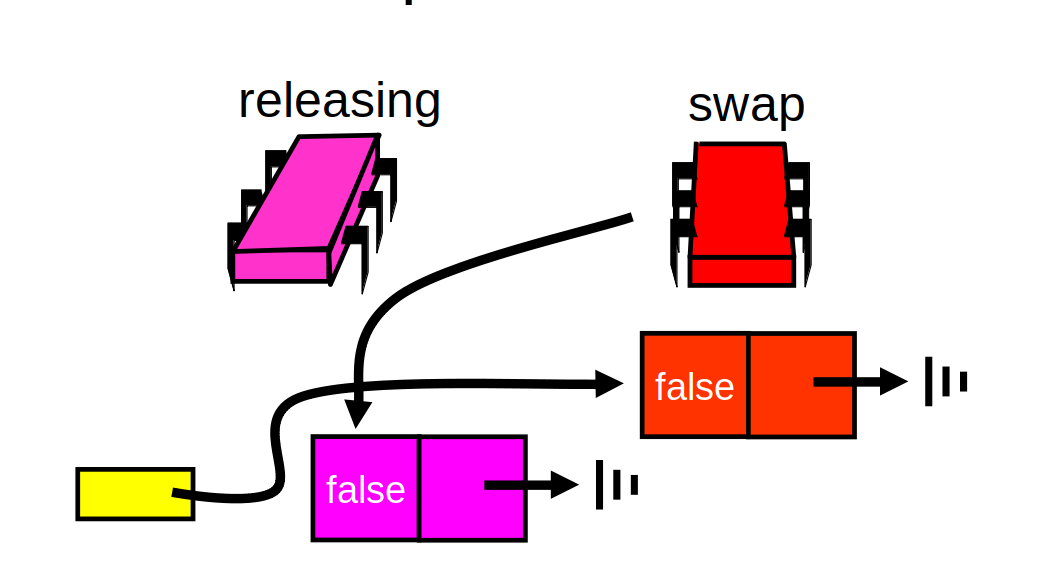
\includegraphics[width=0.7\textwidth]{./pics/mcs-handoff/174.png} \end{center} }
\only<2>{ \begin{center} 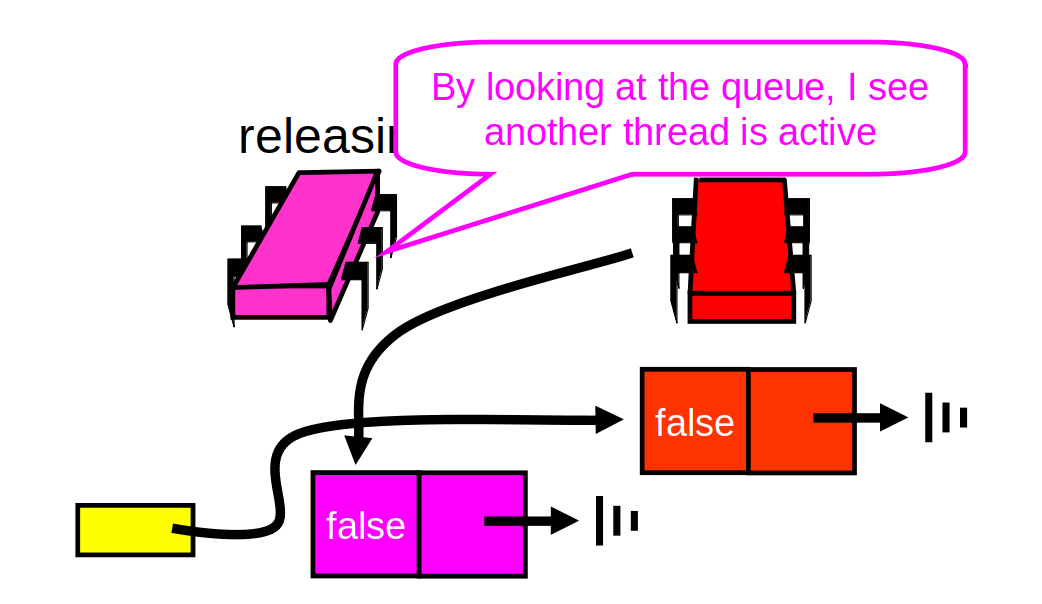
\includegraphics[width=0.7\textwidth]{./pics/mcs-handoff/175.png} \end{center} }
\only<3>{ \begin{center} 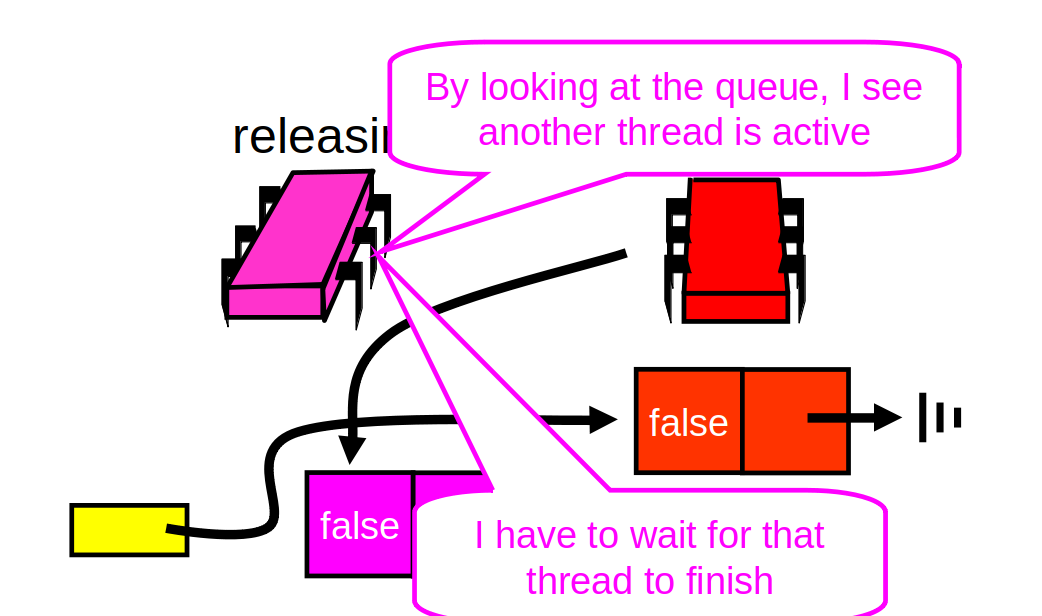
\includegraphics[width=0.7\textwidth]{./pics/mcs-handoff/176.png} \end{center} }
\only<4>{ \begin{center} 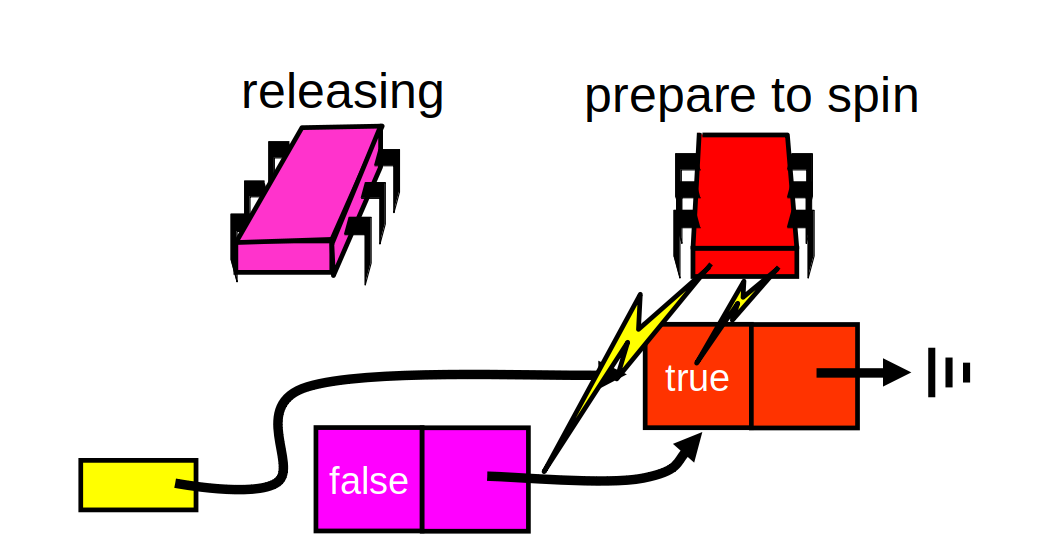
\includegraphics[width=0.7\textwidth]{./pics/mcs-handoff/177.png} \end{center} }
\only<5>{ \begin{center} 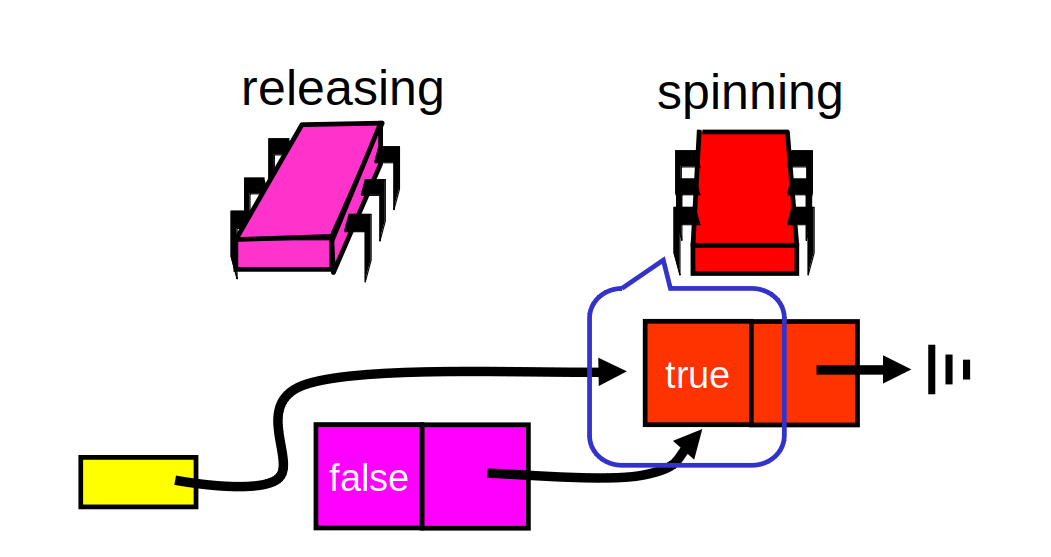
\includegraphics[width=0.7\textwidth]{./pics/mcs-handoff/178.png} \end{center} }
\only<6>{ \begin{center} \includegraphics[width=0.7\textwidth]{./pics/mcs-handoff/179.png} \end{center} }
\only<7>{ \begin{center} \includegraphics[width=0.7\textwidth]{./pics/mcs-handoff/180.png} \end{center} }
\end{frame}

\begin{frame}{MCS: summary}

\textbf{Safety}
\begin{itemize}
  \item Mutual exclusion, Deadlock-freedom, Visibility
\end{itemize}

\textbf{Progress}
\begin{itemize}
  \item Starvation-freedom, \textbf{Fairness} (FIFO)
\end{itemize}

\textbf{Performance}
\begin{itemize}
  \item Memory overhead
  \begin{itemize}
    \item fixed-size node per competitor
    \item $O(L+N)$ where $L$ = number of locks, $N$ = number of threads
  \end{itemize}
  \item Efficiency in contended mode, Scalability
  \begin{itemize}
    \item Third "truly scalable"\ lock in our course
    \item Spins on \textbf{local} memory location
  \end{itemize}  
  \item Backoff policy  
  \begin{itemize}
    \item Spin me right round, baby, right round
  \end{itemize}  
\end{itemize}

\pause

The best lock ever?

\end{frame}


\section{Challenges: interrupt/timeout}
\showTOC

\begin{frame}{Abortable locks}

What if you want to give up waiting for a lock?
\begin{itemize}
  \item Timeout
  \item Database transaction aborted by user
  \item Task of current thread was cancelled
  \pause \item Lecture~\patternsNum: cancellation is useful concurrent pattern
\end{itemize}

\pause
TATAS: just return, no problem

\pause
Queue-based locks: can’t just quit
\begin{itemize}
  \item Thread in line behind will starve
  \item Need a graceful way out
\end{itemize}
\end{frame}


\begin{frame}{Abortable queue locks: problem}

\only<1>{ \begin{center} \includegraphics[width=0.8\textwidth]{./pics/abort/184.png} \end{center} }
\only<2>{ \begin{center} \includegraphics[width=0.8\textwidth]{./pics/abort/185.png} \end{center} }
\only<3>{ \begin{center} \includegraphics[width=0.8\textwidth]{./pics/abort/186.png} \end{center} }
\only<4>{ \begin{center} \includegraphics[width=0.8\textwidth]{./pics/abort/187.png} \end{center} }
\only<5>{ \begin{center} \includegraphics[width=0.8\textwidth]{./pics/abort/188.png} \end{center} }
\only<6>{ \begin{center} \includegraphics[width=0.8\textwidth]{./pics/abort/189.png} \end{center} }
\only<7>{ \begin{center} \includegraphics[width=0.8\textwidth]{./pics/abort/190.png} \end{center} }
\only<8>{ \begin{center} \includegraphics[width=0.8\textwidth]{./pics/abort/191.png} \end{center} }
\only<9>{ \begin{center} \includegraphics[width=0.8\textwidth]{./pics/abort/192.png} \end{center} }

\end{frame}

\begin{frame}{Abortable queue locks: solutions}

\begin{itemize}
  \pause
  \item Exist \pause for some algorithms 
  \pause
  \item Have advantages and disadvantages
  \pause
  \item Add complexity
\end{itemize}

\pause
See Section 7.6 "A Queue Lock with Timeouts" \ in "The Art of Multiprocessor Programming" 

\pause
We will highly appreciate if you will not do THIS in your 3rd critical task

\end{frame}

\section{Challenges: memory management}
\showTOC

\begin{frame}[t]{Reusing node from queue-based lock}

Common problems with memory management in concurrent environments
\begin{itemize}
  \pause \item ABA problem  
  \begin{itemize}
    \pause \item reused node makes some \texttt{CAS} operation to succeed
    \pause \item which is incorrect, "identity" \ of node changed (it is "other" \ node)
  \end{itemize}  
\end{itemize}
\end{frame}

\begin{frame}[t,noframenumbering]{Reusing node from queue-based lock}

Common problems with memory management in concurrent environments
\begin{itemize}
  \item ABA problem  
  \pause \item Inconsistent state (pending write)
  \begin{itemize}
    \pause \item Thread A observed node as "previous" \ in queue
    \begin{itemize}
      \pause \item saved to local variable
      \pause \item plan to write \texttt{node.locked = false}
      \pause \item context switch
     \end{itemize}
    \pause \item Thread B advanced queue, marked node as removed
    \pause \item Thread C reused node: \texttt{node.locked = true}
    \pause \item Thread A wake-ups and "spoils" \ node    
  \end{itemize}
  
\end{itemize}
\end{frame}

\begin{frame}[t,noframenumbering]{Reusing node from queue-based lock}

Common problems with memory management in concurrent environments
\begin{itemize}
  \item ABA problem  
  \item Inconsistent state (pending write)
  \pause \item Use-after-free
  \begin{itemize}
    \pause  \item Thread A published thread-local node
    \pause  \item Thread B observed node as "previous" \ in queue
    \begin{itemize}
      \pause  \item saved to local variable
      \pause  \item plan to read
      \pause \item context switch
     \end{itemize}
    \pause  \item Thread A entered lock
    \pause  \item Thread A released lock
    \pause  \item Thread A finished
    \pause  \item Thread B reads from already freed memory
  \end{itemize}
\end{itemize}
\end{frame}


\begin{frame}[t,noframenumbering]{Reusing node from queue-based lock}

Common problems with memory management in concurrent environments
\begin{itemize}
  \item ABA problem
  \item Inconsistent state (pending write)
  \item Use-after-free
  \pause
  \item Many more...
\end{itemize}
\end{frame}


\begin{frame}[t,noframenumbering]{Reusing node from queue-based lock}

Common problems with memory management in concurrent environments
\begin{itemize}
  \item ABA problem, Inconsistent state (pending write), Use-after-free, ...
\end{itemize}

\pause
Automatic memory management tremendously simplify development of concurrent algorithms

\begin{itemize}
  \pause \item There are implementations of CLH/MCS with node reuse\footnote<3->{Chapter 7 in "The Art of Multiprocessor Programming"}
  \pause \item Developing custom algorithms is hard \pause see KSUH story
  \begin{itemize}
    \item Hydraconf "Java Path Finder: going to Mars without bugs and deadlocks"\footnote<5->{\tiny\url{https://youtu.be/dgHbSL_aDs0?si=vi81xieQ4zKRECQG}}
    \item Heisenbug "Java Path Finder: летим на Марс без багов и дедлоков"\footnote<5->{\tiny\url{https://youtu.be/sQSwShW_IlI?si=ZMlKKLQxMZYhk1T7}}
  \end{itemize}
\end{itemize}
\end{frame}

\begin{frame}[t,noframenumbering]{Reusing node from queue-based lock}

Common problems with memory management in concurrent environments
\begin{itemize}
  \item ABA problem, Inconsistent state (pending write), Use-after-free, ...
\end{itemize}

Automatic memory management tremendously simplify development of concurrent algorithms

\begin{itemize}
  \item There are implementations of CLH/MCS with node reuse
  \item Developing custom algorithms is hard 
\end{itemize}
\pause

My opinion: \textbf{advanced} concurrency in languages with manual memory management is forbidden forest for you
\begin{itemize}
  \pause \item "Atomic weapons" \ from Herb Sutter is a good way to dive in\footnote<3->{\tiny\url{https://youtu.be/A8eCGOqgvH4}}
  \pause \item Using \texttt{std::shared\_ptr} everywhere could be a bad idea\footnote<4->{\tiny\url{https://pvs-studio.ru/ru/blog/posts/cpp/1174/#ID1DE383AA76}}
\end{itemize}

\end{frame}


\section{Spin-then-park}
\showTOC

\begin{frame}[fragile]{Backoff policy revisited}

\begin{minted}{java}
class TATAS_Exponential_Backoff {  
  void lock() {
    int delay = MIN_DELAY;
    while (true) {
      while (state.get() == LOCKED) {} // read-only polling
      if (lock.getAndSet(LOCKED) == UNLOCKED) return; // return on success
      sleep(random() % delay); // delay next write request on failure
      delay = Math.min(delay * 2, MAX_DELAY); // keep delay within bounds    
    }}
  void unlock() { state.set(UNLOCKED); }
}
\end{minted}

\pause 
Trade-off: time-to-react (latency) vs throughput (CPU)

\pause 
\textbf{Idea:} wake-up as soon as lock ready but not earlier

\end{frame}

\questiontime{Which concurrent primitive helps one thread to inform other thread that some event has happened?}

\begin{frame}[fragile]{Spin-then-park: idea}

\texttt{LockSupport.park, LockSupport.unpark}\footnote{\tiny\url{https://docs.oracle.com/en/java/javase/11/docs/api/java.base/java/util/concurrent/locks/LockSupport.html}}

\begin{minted}{java}
boolean tryLock() { return lock.getAndSet(LOCKED) == UNLOCKED; }
void lock() {
  try { while (true) { 
    for (int i = 0; i < SPIN; i++) { if (tryLock()) return; }    
    enterSet.registerWaiter(currentThread()); // "wake-up me on unlock"
    currentThread().park(); // sleep 
  }} finally { enterSet.removeIfPresent(currentThread()); }}
void unlock() { 
  state.set(UNLOCKED); 
  enterSet.unparkAllWaiters(); } // wake-up all registered threads
\end{minted}

\pause
Do you see thundering herd problem here?

\end{frame}

\begin{frame}[fragile]{Spin-then-park: idea}

\begin{minted}{java}
boolean tryLock() { return lock.getAndSet(LOCKED) == UNLOCKED; }
void lock() {
  try { while (true) { 
    for (int i = 0; i < SPIN; i++) { if (tryLock()) return; }    
    enterSet.registerWaiter(currentThread()); // "wake-up me on unlock"
    currentThread().park(); // sleep 
  }} finally { enterSet.removeIfPresent(currentThread()); }}
void unlock() { 
  state.set(UNLOCKED); 
  enterSet.unparkOneWaiter(); } // wake-up one of registered threads
\end{minted}

\pause 
Do you see race condition here?

\end{frame}


\begin{frame}{Check-then-act race condition}

Race condition: 
\begin{itemize}
 \item Thread A sees occupied lock (\texttt{check}), decides to park
 \item Thread B releases lock, notifies all pending threads (e.g. nobody)
 \item Thread A sleeps on condition variable (\textt{act})
\end{itemize}

\end{frame}

\questiontime{Concurrent protocol "fires" \ message in inappropriate time (when \texttt{EnterSet} is empty). How do we call it?}

\begin{frame}[t]{Check-then-act}

One of the most common high-level errors in concurrent algorithms
\begin{itemize}
 \pause \item Thread A observes system state (\texttt{check})
 \pause \item Thread B changes system state
 \pause \item Thread A does something (\texttt{act}) which is incorrect for new system state 
\end{itemize}

\pause

Solutions:
\begin{itemize}
  \pause \item atomic transaction (check-then-act under lock)
  \begin{itemize}
    \pause \item but we are implementing mutex right now!
  \end{itemize}
  \pause \item use RMW operations (e.g. \texttt{compareAndExchange})
  \begin{itemize}
    \pause \item does not work for compound state (multiple variables)
  \end{itemize}
  \pause \item algorithm tolerates "inconsistent actions"
  \begin{itemize}
    \pause \item "missed signal is not a problem"
  \end{itemize}
  \pause \item rework protocol
  \begin{itemize}
    \pause \item "never miss signal"
  \end{itemize}
\end{itemize}
\end{frame}

\begin{frame}[t,fragile]{Spin-then-park with timeouts}

"Missed signal is not a problem"

\begin{minted}{java}
void lock() {
  try { while (true) { 
    for (int i = 0; i < SPIN; i++) { if (tryLock()) return; }    
    enterSet.registerWaiter(currentThread()); // "wake-up me on unlock"
    currentThread().park(1_000); // fixed time sleep 
  }} finally { enterSet.removeIfPresent(currentThread()); }}
void unlock() { 
  state.set(UNLOCKED); 
  enterSet.unparkOneWaiter(); } // wake-up one of registered threads
\end{minted}

\pause
Problem: many waiting threads will repeatedly wake-up and sleep

\end{frame}

\begin{frame}[fragile]{Spin-then-park with double check}

"Never miss signal"

\begin{minted}{java}
void lock() {
  try { while (true) { 
    for (int i = 0; i < SPIN; i++) { if (tryLock()) return; }    
    enterSet.registerWaiter(currentThread()); // "wake-up me on unlock"
    if (tryLock()) return;  // maybe unlock happened before register?
    currentThread().park(); // sleep and be sure not to miss notification
  }} finally { enterSet.removeIfPresent(currentThread()); }}
void unlock() { 
  state.set(UNLOCKED); 
  enterSet.unparkOneWaiter(); } // wake-up one of registered threads
\end{minted}

\pause

Requires intricate reasoning for all possible interleavings of
\begin{itemize}
  \item \texttt{tryLock}, \texttt{registerWaiter}, \texttt{park}, \texttt{unparkOneWaiter}
\end{itemize}
and assumes all of them are linearizable

% Homework
% could we move `get queue` inside the critical section? (swap lines nnn/qqq)
% could we avoid `recheck` (delete line ttt)?

\end{frame}

\section{Summary}

\begin{frame}{Summary}

Advanced alternatives for single-location TATAS
\begin{itemize}
  \item Array-based lock: Anderson Queue Lock (spin on cache line indexed by \texttt{AtomicInteger})
  \item Queue-based lock: CLH (spin on remote location, implicit linked list)
  \item Queue-based lock: MCS (spin on local location, explicit linked list)
\end{itemize}

Challenges with advanced locks
\begin{itemize}
  \item cancellation/timeout support
  \item manual memory management
\end{itemize}

Spin-then-park optimization
\begin{itemize}
  \item Better utilization of CPU and scheduling quantum
  \item Check-then-act race conditions should be avoided in implementation
\end{itemize}

\end{frame}


% \section{Taxonomy of parallel/concurrent problems}
% 
% 
% \begin{frame}{Example with invalid spin lock on weak harwre}
% 
% when release assignment in non-ordered
% 
% \end{frame}
% 
% \begin{frame}{Hard way}
% now every mem barrier (Incl implicit ones) mattern
% 
% there are tools to lower their amount TOOD: publication about auto-removal
% 
% but we will use bullet-proof pattern with acquire-release or full ordering
% 
% \end{frame}
% 
% 
% \begin{frame}{Backoff policies}
% 
% - spin poll
% - sleep poll
% - spin poll then sleep(timeout) then poll 
% 
% tradoff signal speeed/cpu usage
% 
% we need "notify as ready"
% 
% cond vars! or monitors!
% and avoid tthunder herd and stuff
% and avoid race conditions
% 
% \end{frame}
% 
% \begin{frame}{Backoff with sleep}
% incorrect variation
% \end{frame}
% 
% \begin{frame}{Backoff with sleep}
% corrected variation
% 
% conclusion: be aware
% \end{frame}
% 
% \begin{frame}{Backoff with sleep: RAT}
% 
% we suffer some comlexity to be sure that "lost signal" does not happen
% 
% one of possible solutions: timeouts
% 
% lost signal not a problem, but excessive scheduler transfer may arise
% 
% agan tradeoff
% 
% lets minimize it and select only one responsible thread (recently arrived thread, RAT)
% 
% sample with algo
% 
% heuristic idea: simplifies construction, maybe more user friendly for some scenarios, rare negative case, we loose total fairness!
% 
% \end{frame}
% 
% \begin{frame}{Admission policy: queue with slot}
% 
% becuse in practice same thread arrives and arrives, context switching is evil, LIFO is MUCH better throughput than FIFO
% 
% bit fairness is importnat in many domains
% 
% so lets hybrid (eventully FIFO but perf as LIFO)
% 
% it really used (Go shed, etc)
% 
% \end{frame}


% \begin{frame}{Taxonomy of parallel/concurrent problems}
% 
% from publication
% 
% \end{frame}




% \begin{frame}{Work distribution}
% 
% submit/extract/invoke
% classic thread pool
% 
% but tasks could be
% - tiny
% - duynamically create other tasks
% - pulsing behaviour
% - producers are unbalanced
% 
% so we need to distribute it all properly
% 
% 
% work balancing, undersubscription/ooversubscription, useless polling/spinning
% 
% naive solution: queue with mutex
% - obvious inefficiencies
% 
% need variation of striping/replication
% - N queues quite good but termination protocol is hard
% \end{frame}
% 
% \begin{frame}{Work distribution: termination protocol}
% poll N queus and ensure it is empty
% non trivial
% 
% \end{frame}
% 
% \begin{frame}{Work distribution: thread-specific queues}
% 
% every worker has its own queue to avoid contention
% sometimes get work from public repo, sometmies offload tasks to repo
% 
% 
% still have unbalanced scenarios, not full utilization
% \end{frame}
% 
% \begin{frame}{Work distribution: work stealing}
% 
% poll neighbours for available work
% 
% comlexities:
%      task executed only once
%      termination protocol
% 
% \end{frame}
% 
% \begin{frame}{Work distribution: helper threads}
% 
% thread joins for task or pool
% why sleep if you could do the job?
% 
% dynamically-workers pools
% compllexities with works stealing, with stealing topology
% 
% 
% conclusion: you do not know who and when will execute task
% 
% 
% Further reading: kuksenko, Futures/COmpletableFutures and ForkJoinPool design Shipilev
% 
% 
% Basically here we started to talk about user-space scheduling (pros/cons)
% We will have a invited clecture about this., stay tuned
% \end{frame}


\end{document}
